% ============================================================
%  Memoria TFM — Reconstrucción y reparación 3D de objetos rotos
%  Máster en Big Data, Data Science e Inteligencia Artificial
%
%  INSTRUCCIONES PARA COMPILAR EN OVERLEAF:
%    1. Sube este archivo y referencias.bib al proyecto.
%    2. Crea la carpeta "imagenes/" y sube las imágenes del Word
%       con los nombres indicados en cada \includegraphics.
%    3. Compilador: pdfLaTeX (Settings). Bibliografia: BibTeX (no Biber).
% ============================================================

\documentclass[10pt,a4paper]{report}

% ── Codificación y lengua ────────────────────────────────────────────────────
\usepackage[utf8]{inputenc}
\usepackage[T1]{fontenc}
\usepackage[spanish,es-tabla]{babel}
\usepackage{lmodern}
\usepackage{hyphenat}

%\hyphenpenalty=10000
%\exhyphenpenalty=10000
\hyphenpenalty=9000
\exhyphenpenalty=9000
% ── Márgenes ────────────────────────────────────────────────────────────────
\usepackage[top=2cm,bottom=2cm,left=2.2cm,right=2.2cm]{geometry}

% ── Tipografía ───────────────────────────────────────────────────────────────
% microtype desactivado: ralentiza mucho la compilación en Overleaf free
% \usepackage{microtype}
\setlength{\parskip}{6pt}
\setlength{\parindent}{0pt}

% ── Matemáticas ──────────────────────────────────────────────────────────────
\usepackage{amsmath,amssymb}

% ── Gráficos e imágenes ──────────────────────────────────────────────────────
\usepackage{graphicx}
\graphicspath{{imagenes/}}        % busca imágenes en la carpeta imagenes/
\usepackage{float}
\usepackage[labelfont=bf,labelsep=period,font=small]{caption}
\usepackage{subcaption} % para las subfigures apiladas

% ── Tablas ───────────────────────────────────────────────────────────────────
\usepackage{booktabs}
\usepackage{array}
\usepackage{tabularx}
% rotating eliminado — se usa \resizebox en lugar de sidewaystable
\usepackage{threeparttable}   % notas al pie de tabla

% ── Colores ──────────────────────────────────────────────────────────────────
\usepackage[table]{xcolor}
\definecolor{rowgray}{gray}{0.93}

% ── Listas ───────────────────────────────────────────────────────────────────
\usepackage{enumitem}
\usepackage{pifont}
\newcommand{\cmark}{\ding{51}}
\newcommand{\xmark}{\ding{55}}

% ── Encabezados ──────────────────────────────────────────────────────────────
\usepackage{fancyhdr}
\pagestyle{fancy}
\fancyhf{}
\fancyhead[L]{\small\itshape\leftmark}
\fancyhead[R]{\small\thepage}
\renewcommand{\headrulewidth}{0.4pt}

\newcommand{\chapter}[1]{%
  \begingroup
  \let\clearpage\relax
  \chapter{#1}
  \endgroup
}


% ── Formato de títulos (chapter = "1. Título") ───────────────────────────────
\usepackage{titlesec}
\titleclass{\chapter}{straight}
\titleformat{\chapter}[hang]
  {\Large\bfseries}{\thechapter.}{0.7em}{}
\titlespacing*{\chapter}{0pt}{0pt}{8pt}
\titleformat{\section}[hang]
  {\large\bfseries}{\thesection}{0.7em}{}
\titlespacing*{\section}{0pt}{2pt}{4pt}
\titleformat{\subsection}[hang]
  {\normalsize\bfseries}{\thesubsection}{0.7em}{}
\titlespacing*{\subsection}{0pt}{4pt}{3pt}
\titleformat{\subsubsection}[hang]
  {\normalsize\itshape\bfseries}{\thesubsubsection}{0.7em}{}
\titlespacing*{\subsubsection}{0pt}{2pt}{2pt}

% ── Índice de ecuaciones (con tocloft) ───────────────────────────────────────
\usepackage{tocloft}
\newlistof{myequations}{equ}{Índice de ecuaciones}
\newcommand{\myequations}[1]{%
  \addcontentsline{equ}{myequations}{\protect\numberline{\theequation}#1}%
}
\setlength{\cftmyequationsnumwidth}{2.8em}
\renewcommand{\cftmyequationspresnum}{Ec.\,}
\setlength{\cftmyequationsindent}{0pt}

% ── Hipervínculos ────────────────────────────────────────────────────────────
\usepackage[colorlinks=true,
            linkcolor=blue!50!black,
            citecolor=green!40!black,
            urlcolor=blue!70!black]{hyperref}

% ── Bibliografía: natbib + apalike (no requiere biber, mucho más rápido) ─────
\usepackage[authoryear,round,sort]{natbib}

% ── Código ───────────────────────────────────────────────────────────────────
\usepackage{listings}
\lstset{basicstyle=\ttfamily\small, breaklines=true, frame=single,
        backgroundcolor=\color{gray!8}}

% (imágenes gestionadas con graphicspath — todas en imagenes/)

% ============================================================
\begin{document}

% ── Portada ──────────────────────────────────────────────────────────────────
\begin{titlepage}
  \centering
  \vspace*{1cm}
  
\includegraphics[width=15cm]{logo_master}\\[1.5cm]
  {\large Máster en Big Data, Data Science e Inteligencia Artificial}\\[0.4cm]
  {\large Trabajo Fin de Máster}\\[2.5cm]
  {\LARGE\bfseries IA Generativa para la reconstrucción 3D y \\[0.3cm] restauración virtual de objetos}\\[3cm]
  % Foto del objeto (opcional): \includegraphics[width=6cm]{portada_foto}\\[2cm]
  {\large\textbf{Autores}}\\[0.5cm]
  {\large
    Almudena Borreguero Nava\\
    Álvaro Cañete Martí\\
    Luis Carlos Corchuelo Segura\\
    Raquel Roca Pereira\\
    Rocío Sánchez Moreno\\
  }

  \vspace{4cm}
  {\large Madrid, septiembre de 2026}
\end{titlepage}

% ── Índices ──────────────────────────────────────────────────────────────────
\pagenumbering{roman}
\tableofcontents
\newpage
\listoffigures
\newpage
\listoftables
\newpage


\pagenumbering{arabic}
% ============================================================
\chapter{Introducción y motivación}
\label{ch:intro}

Muchos objetos de valor, piezas industriales descatalogadas, componentes dañados en
producción o fragmentos arqueológicos llegan a nuestras manos incompletos.
Una pieza de recambio deja de fabricarse y solo queda un ejemplar roto como referencia, un componente se daña en la cadena de producción y hay que decidir si es reparable o
cuánto material falta.
En estos casos, saber qué forma tenía originalmente el objeto es el primer paso para
actuar sobre él, ya sea para reimprimirlo en~3D, mecanizarlo de nuevo o simplemente
documentarlo.
Tradicionalmente, esta tarea recae en la experiencia de técnicos y especialistas, que
reconstruyen la geometría faltante de forma manual apoyándose en su conocimiento del
objeto y en piezas de referencia similares.
Un proceso lento, costoso y difícil de escalar.

En paralelo, la visión por computador ha avanzado en la dirección opuesta: en lugar de
restaurar lo que falta, ha aprendido a reconstruir en~3D lo que ya existe.
La reconstrucción tridimensional a partir de imágenes consiste en recuperar la forma de
un objeto a partir de una o varias fotografías, y durante décadas se ha
abordado con técnicas geométricas como la estructura a partir de movimiento
(\textit{structure from motion}) o el estéreo.
En los últimos años, sin embargo, los modelos de aprendizaje profundo han demostrado ser
capaces de predecir una representación 3D completa de un objeto directamente a partir de
imágenes, aprendiendo patrones de forma a partir de grandes colecciones de ejemplos.

Esta capacidad de generalizar a partir de lo aprendido abre una pregunta interesante:
si un modelo de reconstrucción 3D ha aprendido cómo son los objetos completos de una
categoría, ¿podría usar ese conocimiento para inferir la parte que le falta a un objeto
roto, del mismo modo que un técnico experimentado intuye la forma original de una pieza
fragmentada?
Este trabajo explora precisamente esa cuestión: si un modelo entrenado únicamente con
objetos completos puede aprender a restaurarlos digitalmente, generando la geometría
faltante a partir de imágenes de su estado roto.
Una respuesta afirmativa tendría aplicación directa en el control de calidad industrial
y la fabricación de piezas de recambio; y también, de forma más indirecta, en la
documentación del patrimonio, donde un modelo 3D digital permite estudiar una pieza
fragmentada sin intervenir sobre el objeto original.

La arquitectura empleada en este trabajo para tal objetivo ha sido Pix2Vox++,
una red de reconstrucción 3D basada en redes convolucionales, aplicada sobre vasijas (tazas, botellas, cuencos...) tanto en estado completo como roto.

El proyecto se estructura en dos fases, en las que se abordan los siguientes objetivos:
\begin{itemize}
  \item Evaluar el comportamiento de Pix2Vox++ sobre objetos completos, estudiando el
        efecto del número de vistas de entrada, del \textit{fine-tuning} y de la
        diversidad de categorías de entrenamiento (fase~1,
        Capítulo~\ref{ch:exp_completos}).
  \item Determinar cómo se comporta un modelo entrenado exclusivamente con objetos
        completos al recibir imágenes de un objeto roto (fase~1,
        Capítulo~\ref{ch:geometrias_rotas}).
  \item Crear un modelo de aprendizaje profundo capaz de obtener la representación
        tridimensional completa del objeto reparado, reconstruyendo la parte faltante (fase~2,
        Capítulo~\ref{ch:generativo}).
\end{itemize}

Tras esta introducción, el Capítulo~\ref{ch:conceptos} presenta los conceptos básicos
de reconstrucción 3D y el Capítulo~\ref{ch:datos} describe los datos y el pipeline de
preparación. A continuación, el Capítulo~\ref{ch:malla} describe la conversión de la
nube reparada en una malla imprimible en 3D. Finalmente, el Capítulo ~\ref{ch:conclusiones} recoge las conclusiones del trabajo, sus limitaciones y
las posibles líneas futuras.

El código desarrollado en este trabajo se encuentra disponible en el siguiente repositorio de GitHub:
\begin{quote}
\url{https://github.com/herredoble/TFM-reconstruccion-3D}
\end{quote}



% ============================================================
\chapter{Conceptos básicos de reconstrucción 3D}
\label{ch:conceptos}

En este capítulo se resumen las nociones necesarias sobre representación 3D: las distintas
formas de codificar un objeto tridimensional, cómo se obtiene esa representación a partir
de imágenes y cómo se evalúa su calidad.

% ── 2.1 ─────────────────────────────────────────────────────────────────────
\section{Formas de representar un objeto en 3D}
\label{sec:representaciones}

Existen varias maneras de representar digitalmente un objeto tridimensional.
Las cuatro empleadas en este trabajo son:

\begin{itemize}
  \item \textbf{Malla (\textit{mesh}):} superficie formada por vértices, aristas y caras triangulares que envuelven el objeto. Es la representación más habitual en programas de diseño 3D y la empleada en los archivos \texttt{.ply} de este proyecto.

  \item \textbf{Nube de puntos:} conjunto de puntos en el espacio con coordenadas
        $X, Y, Z$, sin conectividad entre ellos.

  \item \textbf{Vóxel:} el equivalente tridimensional de un píxel.
        El espacio se divide en una rejilla regular (en este trabajo de $32\times32\times32$
        celdas) y cada celda queda ``ocupada'' o ``vacía''.
        Es la representación que predice el modelo Pix2Vox++ y la usada como referencia del objeto real (\textit{ground truth}) durante el entrenamiento.
        El formato binvox, utilizado en este trabajo, almacena estas rejillas
        de vóxeles de manera óptima.

  \item \textbf{STL (\textit{Standard Tessellation Language}):} formato de malla
        simplificado orientado a la fabricación aditiva.
        A diferencia de los archivos \texttt{.ply}, que pueden incluir color, textura y otras propiedades por vértice, STL solo almacena triángulos (cada cara con sus tres vértices y su normal), sin relaciones de
        adyacencia entre ellos.
        Para que una pieza sea imprimible, la malla debe ser \textit{watertight} (cerrada, sin huecos), condición que garantiza que el interior del objeto queda completamente definido. Es el formato de salida de la segunda fase de este proyecto.
\end{itemize}

\begin{figure}[H]
  \centering
  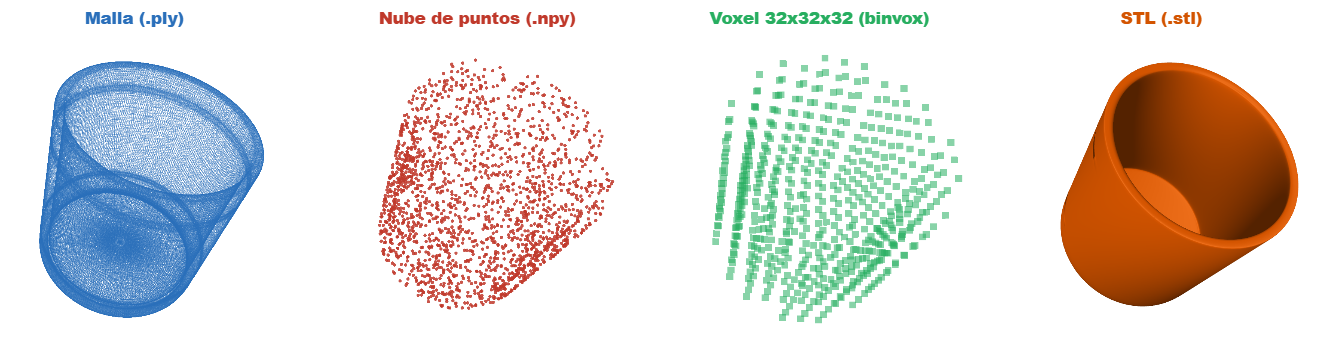
\includegraphics[width=0.75\linewidth]{figura_representaciones}
  \caption{El mismo objeto (taza) en las cuatro representaciones empleadas en el pipeline: malla (.ply), nube de puntos (.npy), vóxel (binvox) y STL (.stl).}
  \label{fig:representaciones}
\end{figure}

% ── 2.2 ─────────────────────────────────────────────────────────────────────

\section{Evaluación de una reconstrucción óptima}
\label{sec:metricas}

Las métricas empleadas a lo largo del trabajo para evaluar la calidad de las
reconstrucciones 3D son las siguientes.

\subsubsection*{Intersección sobre Unión (IoU)}
Solapamiento entre el volumen de vóxeles predichos ($V_{\text{pred}}$) y el real
($V_{\text{gt}}$).
Varía entre 0 (ninguna coincidencia) y~1 (predicción perfecta).
Es la métrica principal en la fase 1 y se define como
\begin{equation}
  \mathrm{IoU} = \frac{|V_{\text{pred}} \cap V_{\text{gt}}|}
                      {|V_{\text{pred}} \cup V_{\text{gt}}|}
  \label{eq:iou}
\end{equation}
\myequations{Intersección sobre Unión (IoU)}



\subsubsection*{Distancia de Chamfer (CD-L1)}
Media de las distancias mínimas entre dos nubes de puntos en ambas direcciones.
Un valor menor indica superficies más parecidas.
Es la métrica principal en la segunda fase del trabajo. Se define como
\begin{equation}
  \mathrm{CD}(P,Q) =
    \frac{1}{|P|}\sum_{p \in P}\min_{q \in Q}\|p-q\|_2 +
    \frac{1}{|Q|}\sum_{q \in Q}\min_{p \in P}\|q-p\|_2
  \label{eq:chamfer}
\end{equation}
\myequations{Distancia de Chamfer (CD-L1)}

donde $P$ y $Q$ representan las nubes de puntos reconstruida y de referencia,
respectivamente, $p \in P$ y $q \in Q$ son puntos individuales de cada nube,
$\|\cdot\|_2$ denota la distancia euclídea y $|P|$ y $|Q|$ representan el
número de puntos de cada nube.

\subsubsection*{Coeficiente de Sørensen-Dice (DSC)}
Compara el doble de la intersección con la suma de los vóxeles ocupados en el volumen
predicho y en el real.
Varía entre 0 y~1; complementa al IoU siendo más sensible en zonas de alto solapamiento. Usando la misma notación que en las métricas anteriores, se define como:
\begin{equation}
  \mathrm{DSC} = \frac{2\,|V_{\text{pred}} \cap V_{\text{gt}}|}
                      {|V_{\text{pred}}| + |V_{\text{gt}}|}
  \label{eq:dice}
\end{equation}
\myequations{Coeficiente de Sørensen-Dice (DSC)}


\subsubsection*{Precisión vóxel}
Proporción de vóxeles predichos como ocupados que pertenecen realmente al objeto.
Un valor bajo indica que el modelo genera volumen de más (falsos positivos). Usando la misma notación que en las métricas anteriores, se define como:
\begin{equation}
  \mathrm{Prec}_{\text{vox}} = \frac{|V_{\text{pred}} \cap V_{\text{gt}}|}{|V_{\text{pred}}|}
  \label{eq:prec_vox}
\end{equation}
\myequations{Precisión vóxel}


\subsubsection*{Recall vóxel}
Proporción del objeto real que ha sido reconstruido.
Un valor bajo indica que el modelo omite partes de la geometría (falsos negativos). Usando la misma notación que en las métricas anteriores, se define como:
\begin{equation}
  \mathrm{Rec}_{\text{vox}} = \frac{|V_{\text{pred}} \cap V_{\text{gt}}|}{|V_{\text{gt}}|}
  \label{eq:rec_vox}
\end{equation}
\myequations{Recall vóxel}

\subsubsection*{F-Score}
Media armónica de la precisión y el recall, que proporciona una medida conjunta
de la calidad de la reconstrucción. Usando la misma notación que en las métricas anteriores, se define como:

\begin{equation}
  F\text{-Score} = \frac{2\cdot\mathrm{Prec}\cdot\mathrm{Rec}}
                          {\mathrm{Prec}+\mathrm{Rec}}
  \label{eq:fscore}
\end{equation}
\myequations{F-Score}



% ── 2.4 ─────────────────────────────────────────────────────────────────────
\section{Modelos de aprendizaje profundo empleados en el pipeline}
\label{sec:modelos_pipeline}

El pipeline integra cuatro modelos preentrenados: uno para la reconstrucción de objetos completos (Pix2Vox++, fase~1), y tres para la
reparación generativa de la nube de puntos (PCN, TopNet y PoinTr, fase~2). Se describen brevemente a continuación:

\subsection{Pix2Vox++ (Reconstrucción 3D multi-vista)}
\label{subsec:pix2vox_modelo}
Arquitectura CNN de tipo \textit{encoder-decoder} con módulos \textit{Merger} y \textit{Refiner} \citep{xie2020pix2vox}. Recibe $N$ imágenes RGB del objeto de $224\times224$ píxeles y genera una rejilla de $32^3$ vóxeles, estimando para cada uno su probabilidad de ocupación. Se organiza en cuatro módulos encadenados: un \textit{encoder} que extrae características visuales de cada imagen y puede emplear diferentes arquitecturas, en este trabajo se utiliza principalmente ResNet-50, y se prueba EfficientNet-B4 como alternativa; un \textit{decoder} que convierte esas características en un volumen preliminar por vista; un \textit{Merger}, que con varias vistas decide qué partes de cada volumen son más fiables y las combina en uno solo, en lugar de promediarlas; y un \textit{Refiner}, que corrige el volumen fusionado suavizando errores y mejorando detalles finos. Se parte del modelo preentrenado en ShapeNet, realizando un \textit{fine-tuning} posterior sobre vasijas.

\subsection{PCN (Point Completion Network)}
\label{subsec:pcn_modelo}
Encoder tipo PointNet~\citep{qi2017pointnet}: cada punto de la nube parcial pasa por
una pequeña red neuronal (MLP) y después
toda la información se combina en un único vector de 1.024 valores que resume la forma
global del objeto (\textit{max-pooling}). A partir de ese vector, un decoder tipo
FoldingNet genera la nube completa en dos etapas: primero
una nube gruesa que aproxima la forma general, y después la expande deformando una
superficie plana hasta ajustarla a la forma
reconstruida (\textit{folding}). En este trabajo se ha adaptado la
resolución de salida a 2.048 puntos, para que
coincida con la resolución empleada en el resto del pipeline, con una etapa gruesa de
512 puntos.

\subsection{TopNet (Decoder jerárquico en árbol)}
\label{subsec:topnet_modelo}
Comparte el mismo encoder que PCN: la nube parcial de 2.048 puntos se resume en un
vector global de 1.024 valores mediante MLPs y max-pooling. Cambia, en cambio, el
decoder: en lugar de generar la nube completa a partir de una única superficie 2D como
PCN, organiza la generación de puntos en forma de árbol. El vector global actúa como
raíz, y en cada nivel del árbol pequeñas redes deciden en qué nuevas ramas se divide
cada punto, hasta llegar a las hojas, que son los puntos finales de la nube completa;
en cada nivel se vuelve a consultar el vector global, para no perder la referencia de
la forma global del objeto \citep{tchapmi2019topnet}. En este trabajo el árbol tiene
cuatro niveles: parte de 8 raíces, que se ramifican sucesivamente hasta 64, después
512 y finalmente 2.048 puntos hoja. Esta estructura en árbol evita que todo el detalle
salga de una única superficie 2D de \textit{folding}, permitiendo representar
geometrías con topologías más complejas a distintas escalas.

\subsection{PoinTr (Point Transformer)}
\label{subsec:pointr_modelo}
Trata la completación como una tarea \textit{sequence-to-sequence} entre grupos de
puntos \citep{yu2021pointr}. Primero, la nube parcial de 2.048 puntos se agrupa en
pequeños conjuntos de puntos cercanos entre sí, y cada grupo se convierte en un vector que resume esa zona local de la nube mediante
DGCNN, una red que construye estas características comparando
cada punto con sus ``vecinos'' más próximos. Un
\textit{transformer} combina esos tokens entre sí junto con unos
\textit{proxy points} (posiciones donde el modelo estima que debería haber puntos, en
la zona rota), permitiendo que cada grupo tenga en cuenta al resto para decidir cómo
rellenar el hueco. A partir de ahí, una parte de la red genera una nube preliminar, que
un FoldingNet local expande hasta la nube completa de 2.048 puntos. 

% ============================================================
\chapter{Datos y pipeline de preparación}
\label{ch:datos}

El entrenamiento de modelos de aprendizaje profundo para la reconstrucción tridimensional
requiere un conjunto de datos rigurosamente estructurado y preprocesado.
En este capítulo se describe el origen de los modelos 3D utilizados, los criterios de
filtrado y las transformaciones necesarias para adaptar la información geométrica a los
formatos de entrada y salida (\textit{ground truth}) de la red neuronal.

% ── 3.1 ─────────────────────────────────────────────────────────────────────
\section{Origen y estructura de los datos}
\label{sec:datos_origen}

Usaremos tres bases de datos para este trabajo: ShapeNetCore, Objaverse y
Fantastic Breaks. Las dos primeras se emplean para generar modelos completos
y roturas sintéticas, mientras que Fantastic Breaks proporciona pares reales
de objetos rotos y completos.


\subsubsection*{ShapeNetCore \textnormal{\citep{chang2015shapenet}}}
Es un repositorio de más de 51.000 modelos poligonales distribuidos en 55 categorías de objetos cotidianos.
Este trabajo acota el estudio a la categoría de vasijas: objetos con concavidades,
asas y topologías variadas, elegidos porque ShapeNetCore ofrece un volumen suficientemente
amplio de muestras para esta clase.
La hipótesis de partida es que, si el pipeline demuestra una reconstrucción precisa y
generalizable sobre esta familia de objetos, la misma metodología sería extrapolable a
cualquier otra categoría geométrica con volumen de datos equivalente.

De los modelos originales se descartaron mallas degeneradas o demasiado simples (menos
de 1.000 caras) y se simplificaron topológicamente aquellas excesivamente pesadas (más
de 200.000 caras).
Además, cada malla fue trasladada para alinear su centroide con el origen de coordenadas
y se escaló proporcionalmente para encajar en un volumen unitario. Este conjunto se emplea en la primera fase del proyecto (Capítulos~\ref{ch:exp_completos}
y~\ref{ch:geometrias_rotas}) para entrenar y evaluar Pix2Vox++ sobre objetos completos
y sobre geometrías rotas.
El resultado son 2.170 mallas limpias y normalizadas en formato \texttt{.ply},
distribuidas como se muestra en la Tabla~\ref{tab:shapenet}.

\begin{table}[H]
  \centering
  \begin{threeparttable}
  \begin{tabular}{ll}
    \toprule
    Categoría & N.º objetos \\
    \midrule
    Jarra / tarro & 545 \\
    Maceta        & 489 \\
    Botella       & 453 \\
    Cubo de basura & 277 \\
    Taza          & 172 \\
    Cuenco        & 146 \\
    Lata          & 88 \\
    \midrule
    \textbf{Total} & \textbf{2.170} \\
    \bottomrule
  \end{tabular}
  \end{threeparttable}
  \caption{Distribución de modelos ShapeNet por categoría de vasijas.}
  \label{tab:shapenet}
\end{table}


\subsubsection*{Objaverse \textnormal{\citep{deitke2023objaverse}}}
Es un repositorio de código abierto con más de 800.000 modelos 3D anotados, de calidad
y estilo muy heterogéneos.
A diferencia de ShapeNet, no está organizado en categorías rígidas: los objetos provienen
de artistas y estudios de diseño, lo que aporta mayor variedad geométrica y visual.
De este repositorio se seleccionaron y limpiaron 131 mallas de la supercategoría de
vasijas (tazas, jarras, cuencos), aplicando los mismos criterios de filtrado que para ShapeNet (mínimo 1.000 caras, centrado y escala unitaria).
Estos modelos se emplean exclusivamente como objetos completos para generar roturas
sintéticas adicionales ya que no existen pares de rotura reales en Objaverse.

\subsubsection*{Fantastic Breaks \textnormal{\citep{lamb2023fantastic}}}
Es el único de los tres \textit{datasets} que ofrece pares reales (fragmento roto,
objeto completo) en lugar de roturas sintéticas.
Contiene 150 objetos domésticos físicamente rotos, escaneados en 3D junto con sus
contrapartes completas mediante un escáner de luz estructurada.
Las nubes de puntos resultantes presentan ruido de escáner, densidad irregular y pequeñas
inconsistencias de alineación entre el fragmento y el objeto completo.
De este conjunto se filtraron los pares de la supercategoría de vasijas (\textit{mug,
bowl, jar, cup}), obteniendo 61 pares utilizables.
La alineación previa de cada par se realizó aplicando la transformación incluida en los
metadatos del \textit{dataset} y refinándola con ICP (\textit{Iterative Closest Point}),
un algoritmo que ajusta iterativamente la posición de una nube de puntos sobre la otra
hasta minimizar la distancia entre ambas superficies, ya que fragmento y objeto completo
provienen de escaneos independientes.
Dado su tamaño reducido (61 pares frente a los 2.501 pares sintéticos del \textit{dataset}
final de entrenamiento, Sección~\ref{sec:datos_e3}), se usa principalmente como conjunto
de evaluación en condiciones reales y, de forma experimental, como datos de entrenamiento adicional.

% ── 3.2 ─────────────────────────────────────────────────────────────────────
\section{Conversión de la malla al \textit{ground truth}: de PLY a binvox}
\label{sec:ply_binvox}

Como se ha comentado, la base de datos principal de la fase 1, ShapeNetCore,
se guarda en formato \texttt{.ply}. Sin embargo, dado que la arquitectura de
reconstrucción empleada en este trabajo, Pix2Vox++, predice una rejilla
volumétrica binaria y no una malla, cada modelo se convirtió en un volumen
\texttt{model.binvox} de resolución $32\times32\times32$ mediante la herramienta
binvox. El proceso solidifica el interior del objeto,
deteniendo el llenado un vóxel antes de alcanzar la superficie de la malla
(evitando así huecos internos), y se complementa con un renderizado adicional
en modo contorno que preserva partes finas y estrechas, como las asas, que de
otro modo desaparecerían al reducir la resolución a $32^3$
(Figura~\ref{fig:binvox}).

El objeto se centra siempre en la misma posición del cubo de vóxeles,
garantizando la correspondencia espacial con las imágenes de entrada. Los
datos resultantes, comprimidos mediante \textit{run-length encoding}, se
descomprimen y se transponen del orden interno de binvox ($X,Z,Y$) al orden
($X,Y,Z$) que espera Pix2Vox++.

\begin{figure}[H]
  \centering
  \includegraphics[width=0.7\linewidth]{imagenes/figura_3_1_ply_vs_binvox.png}
  \caption{Proceso de voxelización: malla \texttt{.ply} original (izquierda) y
           volumen binvox $32^3$ resultante (derecha).}
  \label{fig:binvox}
\end{figure}

% ── 3.3 ─────────────────────────────────────────────────────────────────────
\section{Generación de datos de entrada: renderizado de vistas 2D}
\label{sec:renderizado}

Por otro lado, ya que Pix2Vox++ requiere imágenes bidimensionales como datos de entrada, se generan
vistas 2D sintéticas mediante BlenderProc~\citep{denninger2020blenderproc}, a partir de los modelos 3D disponibles, garantizando
la correspondencia espacial exacta con el \textit{ground truth}
(Figura~\ref{fig:blenderproc}).
Para que el modelo de aprendizaje profundo se centre de forma exclusiva en la inferencia de la geometría y no sufra sesgos por las
texturas originales de ShapeNet, cada malla se traslada y escala con los mismos parámetros de normalización del \texttt{.binvox} asociado. Además, se aplica un material neutro homogéneo a todos los objetos, con iluminación fija de tres puntos.
Para cada objeto se capturan 20 vistas reproducibles (8 a 20° de elevación, 8 a 40°
y 4 a 60°, radio 2,2), en formato RGBA a $224\times224$\,píxeles, normalizadas después
a $[-1, 1]$.

Este repertorio permite, en capítulos posteriores, evaluar el modelo con distintos números de vistas de entrada
(1, 5 o 20 vistas), tomando siempre subconjuntos fijos y reproducibles del total capturado.

\begin{figure}[H]
  \centering
  \includegraphics[width=0.85\linewidth]{figura_3_3_vistas (2).png}
  \caption{Malla original y las 20 vistas renderizadas generadas con BlenderProc. En rojo: vista usada en los experimentos de 1 vista. En naranja: subconjunto de 5 vistas.}
  \label{fig:blenderproc}
\end{figure}

% ── 3.4 ─────────────────────────────────────────────────────────────────────
\section{División del conjunto de datos}
\label{sec:split}

Los 2.170 objetos validados de ShapeNetCore se dividieron en tres subconjuntos independientes:
entrenamiento (70\,\%), validación (15\,\%) y test (15\,\%).
La partición se realizó a nivel de objeto, no de imagen: las 20 vistas de un mismo
objeto pertenecen de forma indivisible a un único subconjunto, evitando así
\textit{data leakage}.

% ============================================================
\chapter{Experimentación sobre objetos completos}
\label{ch:exp_completos}

Este capítulo evalúa la capacidad de Pix2Vox++ para reconstruir objetos tridimensionales completos a partir de imágenes RGB renderizadas, con el objetivo de determinar cómo influyen tres factores en la calidad de la reconstrucción: el número de vistas disponibles por objeto (1, 5 o 20), la aplicación de \textit{fine-tuning} sobre la categoría objetivo, y la ampliación del conjunto de categorías utilizadas en el entrenamiento.

Todos los experimentos se realizan sobre objetos completos, con sus 20 vistas disponibles y su \textit{ground truth} voxelizado, y mantienen constantes las particiones de entrenamiento, validación y test descritas en el Capítulo ~\ref{sec:split}, evitando fugas de información entre subconjuntos. La Tabla ~\ref{tab:config_experimentos} resume la configuración de cada experimento citado en este capítulo, y sirve de referencia para los siguientes capítulos. 
Además, para garantizar la comparabilidad, se emplean las mismas vistas de referencia en todas las evaluaciones. Sin embargo, los modelos se entrenan con vistas seleccionadas al azar, lo que permite que, en la implementación final, puedan utilizarse cinco vistas cualesquiera de la taza sin comprometer la validez del modelo. 

A continuación, se detallan los resultados de los experimentos más relevantes. 

\begin{table}[H]
  \centering
  \begin{threeparttable}
  \begin{tabular}{lllll}
    \toprule
    Experimento & Vistas & \textit{Fine-tuning} & Categorías & Encoder \\
    \midrule
    1--3   & 1 / 5 / 20 & No  & Taza                    & ResNet-50      \\
    4--6   & 1 / 5 / 20 & Sí  & Taza                    & ResNet-50      \\
    7 & 20        & No  & Taza + Botella          & ResNet-50      \\
    11  & 20        & Sí  & Taza + Botella          & ResNet-50      \\
    9, 10  & 5 / 20        & Sí  & 4 categorías            & ResNet-50      \\
    12     & 5        & Sí  & Taza                    & EfficientNet-B4 \\
    13     & 5          & Sí  & 7 categorías            & ResNet-50      \\
    \bottomrule
  \end{tabular}
  \begin{tablenotes}\footnotesize
    \item El experimento 8 no aparece: fue un intento con \textit{data leakage}, detectado y descartado.
  \end{tablenotes}
  \caption{Configuraciones aplicadas en los experimentos realizados.}
  \label{tab:config_experimentos}
  \end{threeparttable}
\end{table}



% ── 4.1 ─────────────────────────────────────────────────────────────────────
\section{Número de vistas y necesidad de \textit{fine-tuning}}
\label{sec:vistas_finetuning}

Los experimentos 1 a 3 evalúan el modelo preentrenado sin ningún ajuste adicional, sobre la categoría de tazas, con 1, 5 y 20 vistas por objeto respectivamente. Mientras que los experimentos 4 a 6 repiten la misma comparación, pero aplicando en este caso \textit{fine-tuning}, ajustando los pesos del modelo sobre el conjunto de entrenamiento de tazas.
El fine‑tuning incorpora:
\begin{itemize}
  \item Tasas de aprendizaje diferenciadas para \textit{encoder} y \textit{decoders}.
  \item \textit{Batch Normalization} activada en el \textit{encoder}.
  \item Recorte de gradiente (\textit{gradient clipping}) para estabilizar el entrenamiento.
  \item \textit{Scheduler} con reducción de la tasa de aprendizaje cuando la métrica IoU no mejora.
  \item \textit{Early stopping} basado en la validación para evitar sobreajuste.
\end{itemize}


Estas técnicas permiten que el modelo se adapte mejor a la geometría específica de la categoría objetivo. Todos los entrenamientos se ejecutan sobre la GPU A100 de Google Colab, garantizando estabilidad y tiempos de cómputo adecuados. 

En la Tabla~\ref{tab:tabla_resultados_finetuning} se muestran los resultados de los seis primeros experimentos, cuyo objetivo es determinar el número de vistas más adecuado para el modelo y evaluar la necesidad de realizar \textit{fine-tuning} sobre los pesos preentrenados. En la tabla \ref{tab:resultados_finetuning} del Anexo~\ref{ap:tablas}, se muestra información adicional de cada experimento.

\begin{table}[H]
  \centering
  \begin{tabular}{ccccccc}
    \toprule
    Exp. & \textit{Fine-tuning} & Vistas & IoU & Dice & Chamfer & F-score \\
    \midrule
    1 & No & 1  & 0,17  & 0,2823 & 2,4174 & 0,3594 \\
    2 & No & 5  & 0,159 & 0,2606 & 2,6474 & 0,3097 \\
    3 & No & 20 & 0,158 & 0,2608 & 2,7197 & 0,3016 \\
    4 & Sí & 1  & 0,398 & 0,5544 & 1,3218 & 0,6199 \\
    5 & Sí & 5  & 0,534 & 0,6815 & 0,8572 & 0,8016 \\
    6 & Sí & 20 & 0,558 & 0,6968 & 0,8036 & 0,8121 \\
    \bottomrule
  \end{tabular}%
  \caption{Resultados de los experimentos 1--6 para evaluar el efecto del \textit{fine-tuning} y del número de vistas.}
  \label{tab:tabla_resultados_finetuning}
\end{table}

En primer lugar, se evalúa el modelo en configuración \textit{zero-shot}, es decir, sin adaptar sus pesos al problema específico de reconstrucción de tazas, utilizando directamente los modelos preentrenados con ShapeNet. Los experimentos 1--3 muestran un rendimiento reducido para las tres configuraciones de vistas. De hecho, el mejor resultado se obtiene con una única vista, alcanzando un IoU de 0,17 y un F-score de 0,3594. Sin embargo, estos resultados son insuficientes para obtener reconstrucciones de calidad.

Al introducir el \textit{fine-tuning}, se observa una mejora notable en todas las métricas. El experimento 4, correspondiente a una única vista, incrementa el IoU de 0,17 a 0,398. Al aumentar el número de vistas a cinco, los resultados mejoran considerablemente, alcanzando un IoU de 0,534, un Dice de 0,6815 y un F-score de 0,8016. Finalmente, el uso de 20 vistas produce una mejora adicional, aunque más moderada, alcanzando un IoU de 0,558 y un F-score de 0,8121.

Por tanto, los resultados muestran que el \textit{fine-tuning} resulta necesario para adaptar el modelo al dominio específico de las tazas y obtener reconstrucciones de mayor calidad. En cuanto al número de vistas, una única vista queda descartada debido a su menor rendimiento. Aunque 20 vistas proporcionan los mejores resultados, la mejora respecto a cinco vistas es relativamente reducida frente al incremento del coste computacional, al requerir cuatro veces más imágenes de entrada. Por ello, el número de vistas continúa siendo una variable de estudio en los experimentos posteriores, donde se analizará si el incremento en el número de vistas permite obtener mejoras suficientemente significativas como para justificar su mayor coste computacional.


% ── 4.2 ─────────────────────────────────────────────────────────────────────
\section{Ampliación del conjunto de categorías de entrenamiento}
\label{sec:mas_categorias}

Una vez establecido que el \textit{fine-tuning} es necesario, se estudia si ampliar la diversidad geométrica del conjunto de entrenamiento mejora la capacidad de reconstrucción del modelo. Para ello, se incorporan progresivamente nuevas categorías de ShapeNet, partiendo de la configuración específica para tazas utilizada en los experimentos anteriores.

En primer lugar, se incorporan las botellas, dando lugar a una configuración de dos categorías. El experimento 7 evalúa esta configuración sin \textit{fine-tuning}, mientras que el experimento 11 utiliza \textit{fine-tuning} y evalúa tanto el conjunto global como específicamente las tazas. Posteriormente, los experimentos 9 y 10 amplían el entrenamiento a cuatro categorías (tazas, botellas, tarros y cuencos) y permiten estudiar además el efecto de reducir el número de vistas de 20 a 5. Los resultados más relevantes se muestran en la Tabla ~\ref{tab:tabla_resultados_categorias_1}, mientras que en la tabla \ref{tab:resultados_categorias} del ~\ref{ap:tablas}, se muestra información adicional de cada experimento.

\begin{table}[H]
  \centering
  \resizebox{\textwidth}{!}{%
  \begin{tabular}{cccccccccc}
    \toprule
    Exp. & \textit{Fine-tuning} & Test & N categorías & Vistas & N test &
    IoU & Dice & Chamfer & F-score \\
    \midrule
    7  & No  & Global & 2 & 20 & 94  & 0,122 & 0,1977 & 4,1091 & 0,2042 \\
    11 & Sí  & Global & 2 & 20 & 94  & 0,729 & 0,8265 & 0,5663 & 0,8662 \\
    11 & Sí  & Tazas  & 2 & 20 & 26  & 0,568 & 0,7099 & 0,7191 & 0,8285 \\
    9  & Sí  & Global & 4 & 20 & 198 & 0,693 & 0,7977 & 0,6137 & 0,8536 \\
    9  & Sí  & Tazas  & 4 & 20 & 26  & 0,584 & 0,7199 & 0,7148 & 0,8363 \\
    10 & Sí  & Global & 4 & 5  & 198 & 0,702 & 0,8068 & 0,5755 & 0,8674 \\
    10 & Sí  & Tazas  & 4 & 5  & 26  & 0,592 & 0,7287 & 0,6520 & 0,8575 \\
    \bottomrule
  \end{tabular}%
  }
  \caption{Resultados de los experimentos 7, 9, 10 y 11 para diferentes configuraciones de entrenamiento.}
  \label{tab:tabla_resultados_categorias_1}
\end{table}

El experimento 7 confirma que las bajas métricas observadas en la configuración \textit{zero-shot} no se deben al número de categorías, ya que el IoU se mantiene reducido (0,122). Por tanto, ampliar la diversidad del entrenamiento no sustituye la necesidad de realizar \textit{fine-tuning}.

Con \textit{fine-tuning}, la incorporación de nuevas categorías no perjudica el rendimiento sobre las tazas. El experimento 11 alcanza un IoU de 0,568 en la evaluación específica, ligeramente superior al 0,558 obtenido con el entrenamiento exclusivo en tazas. Al ampliar a cuatro categorías, el experimento 9 eleva este valor hasta 0,584, mientras que el IoU global alcanza 0,693.

Finalmente, los experimentos 9 y 10 muestran que reducir las vistas de 20 a 5 no provoca un deterioro del rendimiento. De hecho, el IoU global aumenta de 0,693 a 0,702 y el específico sobre tazas de 0,584 a 0,592. Dado que cinco vistas reducen en un 75\% el número de imágenes procesadas sin pérdida de rendimiento, se adopta esta configuración para los experimentos posteriores, buscando un mejor equilibrio entre calidad de reconstrucción y coste computacional.

% ── 4.3 ─────────────────────────────────────────────────────────────────────
\section{Sustitución de la red neuronal del \textit{encoder}}
\label{sec:encoder_eficientnet}

Una vez fijadas las cinco vistas y ampliado el conjunto de entrenamiento a cuatro categorías, se estudia si la sustitución de ResNet-50, utilizada como \textit{backbone} de Pix2Vox++, por una arquitectura más reciente y eficiente puede mejorar el rendimiento. Para ello, en el experimento 12 se sustituye ResNet-50 por EfficientNet-B4. Los resultados, mostrados en la Tabla~\ref{tab:tabla_resultados_categorias_2}, presentan una ligera disminución en todas las métricas respecto al experimento 11. Además, la sustitución requiere modificaciones en el preprocesamiento y en el propio \textit{pipeline}, debido a que Pix2Vox++ no está diseñada originalmente para trabajar con este \textit{backbone}. Por tanto, se mantiene ResNet-50 para los experimentos posteriores.

Finalmente, en el experimento 13 se amplía el entrenamiento a las siete categorías disponibles, manteniendo ResNet-50 y cinco vistas. Aunque el rendimiento global disminuye ligeramente respecto al obtenido con cuatro categorías, la evaluación específica sobre tazas alcanza los mejores resultados del conjunto de experimentos, con un IoU de 0,606, un Dice de 0,7417 y un F-score de 0,8688. Además, las reconstrucciones obtenidas presentan una mejora visual respecto a las configuraciones anteriores. Estos resultados sugieren que, para el objetivo específico de reconstruir tazas, una mayor diversidad de categorías durante el entrenamiento puede favorecer la reconstrucción de esta clase, por lo que esta configuración se empleará en los experimentos posteriores.

\begin{table}[H]
  \centering
  \resizebox{\textwidth}{!}{%
  \begin{tabular}{cccccccccc}
    \toprule
    Exp. & Modelo & Test & N categorías & Vistas & N test &
    IoU & Dice & Chamfer & F-score \\
    \midrule
    12 & EfficientNet-B4 & Global & 4 & 5 & 198 & 0,661 & 0,7762 & 0,6887 & 0,8292 \\
    12 & EfficientNet-B4 & Tazas  & 4 & 5 & 26  & 0,547 & 0,6913 & 0,7030 & 0,8328 \\
    13 & ResNet-50       & Global & 7 & 5 & 327 & 0,650 & 0,7623 & 0,6855 & 0,8343 \\
    13 & ResNet-50       & Tazas  & 7 & 5 & 26  & 0,606 & 0,7417 & 0,6236 & 0,8688 \\
    \bottomrule
  \end{tabular}%
  }
  \caption{Resultados de los experimentos 12 y 13 para diferentes arquitecturas y categorías de entrenamiento.}
  \label{tab:tabla_resultados_categorias_2}
\end{table}


% ── 4.4 ─────────────────────────────────────────────────────────────────────
\section{Resumen de esta fase}
\label{sec:resumen_exp}

De acuerdo con los resultados anteriores, se selecciona el experimento 13 (5 vistas, \textit{fine-tuning} y siete categorías) como configuración óptima de esta fase, por ofrecer el mejor equilibrio entre coste computacional y calidad de reconstrucción, la IoU más alta tanto en evaluación global como específica sobre tazas, y mayor robustez ante variaciones geométricas gracias al entrenamiento con siete categorías. Esta configuración se utiliza como base para la siguiente fase del trabajo, centrada en la reconstrucción de objetos dañados y en la capacidad de generalización del modelo (Capítulo \ref{ch:generativo}).

\begin{figure}[H]
  \centering
  \begin{tabular}{ccc}
    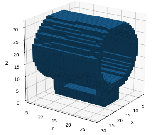
\includegraphics[width=0.25\linewidth]{imagen_taza_real} &
    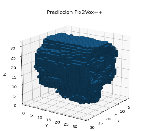
\includegraphics[width=0.25\linewidth]{imagen_pred_exp4} &
    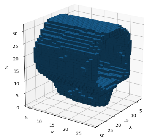
\includegraphics[width=0.25\linewidth]{imagen_pred_exp13} \\
    \small Taza real &
    \small Predicción exp.~4 &
    \small Predicción exp.~13 \\
  \end{tabular}
  \caption{Comparación cualitativa entre una taza real, la predicción del experimento 4 (1 vista, \textit{fine-tuning}, taza) y la predicción del experimento 13 (5 vistas, \textit{fine-tuning}, 7 categorías).}
  \label{fig:comp_exps}
\end{figure}

% ============================================================
\chapter{Evaluación sobre geometrías rotas}
\label{ch:geometrias_rotas}

Una vez seleccionado el modelo óptimo de la fase anterior (experimento 13), se evaluó
su capacidad para generalizar a un escenario radicalmente distinto: geometrías
parcialmente rotas.
El objetivo era comprobar si una red entrenada exclusivamente para reconstruir volúmenes
completos podía inferir correctamente la forma de una pieza rota a partir únicamente de
sus imágenes 2D, y en qué medida un reentrenamiento dirigido podía cerrar esa brecha. La metodología seguida fue incremental, y así se presenta a continuación.

% ── 5.1 ─────────────────────────────────────────────────────────────────────
\section{Metodología con datos reales: BPA y Fantastic Breaks}
\label{sec:bpa_fb}

El enfoque inicial se basó en el conjunto de datos externo Fantastic Breaks,
que contiene nubes de puntos 3D obtenidas de escaneos de tazas reales con fracturas físicas.
Dado que Pix2Vox++ requiere imágenes 2D como entrada, era necesario convertir estas nubes
discontinuas en mallas sólidas \texttt{.ply} renderizables mediante BlenderProc.
Para ello se empleó el algoritmo \textit{Ball Pivoting}~\citep{bernardini1999ball} (BPA), que simula hacer rodar una esfera virtual sobre los puntos para tejer una malla de triángulos entre ellos.

Su aplicación sobre datos reales rotos presentó dos problemas insalvables. Por un lado, BPA no conseguía cerrar de forma natural las transiciones abruptas de la fractura, generando artefactos y defectos topológicos severos. Por otro lado, obtener una malla renderizable sin agujeros exigía aplicar algoritmos de
cierre volumétrico que arreglaban la zona de la rotura, devolviendo a la taza su forma completa original y destruyendo el propósito de la prueba: evaluar al modelo precisamente sobre lo que falta.

% ── 5.2 ─────────────────────────────────────────────────────────────────────
\section{Metodología con roturas sintéticas y \textit{fine-tuning}}
\label{sec:roturas_sinteticas}

Ante la imposibilidad de usar las nubes reales sin distorsionar la geometría, se optó
por generar roturas sintéticas sobre las mallas \texttt{.ply} intactas ya empleadas para
entrenar Pix2Vox++ (172 tazas).
Cada objeto se interseca con un plano 3D de orientación y posición aleatorias, validando
que la pieza resultante conserve entre el 25\% y el 85\% de los vértices originales,
para garantizar que siga siendo reconocible como taza parcialmente destruida.
A diferencia de BPA, este método produce bordes de fractura completamente limpios y
\textit{watertight}, listos para generar de forma fiable las cinco vistas de entrada
(Figura~\ref{fig:rotura_sintetica}).

\begin{figure}[H]
  \centering
  \includegraphics[width=0.75\linewidth]{imagenes/figura_5_1_rotura_sintetica.png}
  \caption{Ejemplo de taza con rotura sintética y sus cinco vistas correspondientes generadas con BlenderProc, a partir de la taza original y su plano de fractura.}
  \label{fig:rotura_sintetica}
\end{figure}

% ── 5.3 ─────────────────────────────────────────────────────────────────────
\section{Resultado: evaluación \textit{zero-shot} y \textit{fine-tuning}}
\label{sec:resultados_roturas}

Sobre este nuevo conjunto, se evaluó primero el modelo del experimento 13, entrenado
exclusivamente con tazas completas, sin ningún ajuste adicional (evaluación
\textit{zero-shot}).
El resultado confirmó una capacidad de generalización prácticamente nula: IoU medio
de~0,054 y Dice de~0,098 sobre las 172 tazas rotas, con el modelo generando volúmenes que ignoran por completo la ausencia de material y tienden a rellenar la forma como si el objeto estuviera intacto.

Se decidió, entonces, adaptar el modelo mediante \textit{fine-tuning}. De las 172 tazas rotas, las 146 destinadas a entrenamiento y validación se ampliaron, generando 532 variantes de rotura adicionales (varias fracturas por objeto, siempre agrupadas por la identidad de la taza original para evitar fugas de información). Las 26 tazas restantes, reservadas como conjunto de test, mantuvieron su única rotura ya evaluada en el paso anterior, permitiendo comparar directamente el mismo caso antes y después del ajuste. Durante el reentrenamiento, se partió del modelo del experimento 13 y se congelaron las estadísticas de las capas de \textit{Batch Normalization}.

La evaluación final sobre las 26 tazas de test (Tabla \ref{tab:roturas}) confirma el efecto de la adaptación: el modelo \textit{fine-tuneado} multiplica por casi seis el IoU del modelo base, y mejora el resultado en 25 de las 26 tazas evaluadas.

\begin{table}[H]
  \centering
  \begin{tabular}{lccc}
    \toprule
    Modelo evaluado & IoU medio & Coef.\ Dice & Mejora (IoU) \\
    \midrule
    Base (solo tazas completas)     & 0,0553 & 0,1009 & --- \\
    \textit{Fine-tuneado} (adaptado a roturas) & 0,3113 & 0,4544 & +0,2560 \\
    \bottomrule
  \end{tabular}
  \caption{Rendimiento comparativo en la reconstrucción de tazas rotas.}
  \label{tab:roturas}
\end{table}

La Figura \ref{fig:comp_finetuning} ilustra este efecto sobre el mismo fragmento generado en la Figura \ref{fig:rotura_sintetica}: mientras que el modelo base apenas reconoce la forma del objeto (IoU~$= 0{,}001$), el modelo ajustado recupera una geometría mucho más cercana a la real (IoU~$= 0{,}625$). 
Pese a la mejora sustancial de ciertos ejemplos, el modelo \textit{fine-tuneado} dista de una reconstrucción perfecta (Dice~$= 0{,}45$). Las limitaciones de este enfoque y las vías para mitigarlas se discuten en el Capítulo \ref{ch:conclusiones}.


\begin{figure}[H]
  \centering
  \includegraphics[width=0.85\linewidth]{imagenes/descarga (1).png}
  \caption{Comparativa visual entre las predicciones del modelo base y el modelo \textit{fine-tuneado} sobre una taza rota del conjunto de test.}
  \label{fig:comp_finetuning}
\end{figure}

% ============================================================
\chapter{Creación del modelo generativo para la reconstrucción del objeto roto}
\label{ch:generativo}

\section{Motivación y enfoque del problema}
\label{sec:motivacion_generativo}

Pix2Vox++ reconstruye la forma \textit{actual} del fragmento, con la región dañada
ausente, incluso en su versión fine-tuneada (Capítulo~\ref{ch:geometrias_rotas}). El
pipeline necesita, en cambio, la geometría \textit{original} del objeto, previa a la
rotura, para poder imprimir la pieza de repuesto.

Esta diferencia (reconstruir lo que hay frente a completar lo que falta) define la
tarea de \textit{shape completion}.
El problema se formula así: dada una nube de puntos parcial que representa un fragmento
de un objeto, predecir la nube de puntos completa del objeto original antes del daño.
Las etapas de preprocesado de imágenes (Capítulo \ref{ch:datos}) y aplicación del modelo Pix2Vox++ (Capítulo \ref{ch:exp_completos}) obtienen la nube parcial a partir de las fotos; mientras que la fase a tratar a continuación, la completa.

\begin{center}
Fotos del objeto roto $\to$
Modelo Pix2Vox++ $\to$ Nube parcial (2.048 pts) $\to$
Modelo generativo (PoinTr) $\to$ Nube completa $\to$
Generación de STL imprimible
\end{center}

El enfoque es supervisado: se entrena con pares (nube rota, nube completa), generando
las nubes rotas sintéticamente para simular la salida esperada.
Se compararon tres arquitecturas de complejidad creciente (PCN, TopNet, PoinTr) con el
mismo \textit{dataset} y protocolo.

\subsection{Conversión de la salida de Pix2Vox++ (vóxeles) a nube de puntos}
\label{subsec:interfaz_e2_e3}

Pix2Vox++ produce como salida una cuadrícula de vóxeles $32^3$.
Este formato no es directamente compatible con la entrada de esta nueva fase, que espera
una nube de 2.048 puntos, cada uno con sus tres coordenadas $(X, Y, Z)$ (un array de forma $(2{.}048, 3)$), centrada en el origen y escalada a esfera unidad.
El paso de conversión tiene cuatro etapas:
\begin{enumerate}
  \item Umbralización: se aplica un umbral de~0,5 sobre la cuadrícula para
        obtener una máscara binaria de ocupación.
  \item Extracción de coordenadas: las celdas ocupadas se convierten en
        puntos 3D.
  \item Normalización: el conjunto se centra en el centroide y se escala a
        esfera unidad.
  \item Submuestreo a 2.048 puntos: como el número de celdas ocupadas varía
        de un objeto a otro, es necesario fijar siempre el mismo número de
        puntos de salida. Si hay más de 2.048 celdas ocupadas, se seleccionan
        2.048 de ellas mediante \textit{furthest point sampling} (FPS): un
        método que, partiendo de un punto al azar, va añadiendo en cada paso
        el punto más alejado de los ya seleccionados, de forma que los puntos
        resultantes queden repartidos de manera uniforme por toda la
        superficie del objeto, en lugar de agruparse en una sola zona.
\end{enumerate}

Esta conversión tiene una limitación: la resolución $32^3$ implica que los puntos del
resultado solo pueden ocupar posiciones múltiplos de $1/32\approx 0{,}031$ unidades.
En objetos con geometría fina (asas, bordes delgados), esto puede perder detalle
geométrico capturado implícitamente por el modelo entrenado.
Esta diferencia de dominio es una fuente de error adicional en producción.

% ── 6.2 ─────────────────────────────────────────────────────────────────────
\section{Datos de entrenamiento para \textit{shape completion}}
\label{sec:datos_e3}

Los \textit{datasets} empleados, ShapeNet, Objaverse y Fantastic Breaks, se describen
en la Sección~\ref{sec:datos_origen}. Para esta fase, el conjunto de
mallas de ShapeNet se depuró más allá del filtrado general del Capítulo~\ref{ch:datos},
descartando adicionalmente figuras sin sentido geométrico al fracturarlas, hasta
quedar en 855 mallas limpias. A partir de estas, y de las mallas de Objaverse, se
generaron varias roturas sintéticas por objeto (Sección~\ref{subsec:roturas_sinteticas_e3}),
obteniendo un total de 2.104 pares de ShapeNet y 397 de Objaverse. Junto con los
61 pares reales de Fantastic Breaks, el \textit{dataset} combinado para esta
fase contiene 2.562 pares.

\subsection{Generación de roturas sintéticas}
\label{subsec:roturas_sinteticas_e3}
Sobre las mallas de ShapeNet y Objaverse (Fantastic Breaks ya aporta roturas reales,
por lo que no se procesa en este paso), se genera una rotura sintética partiendo de
una nube densa de 20.000 puntos por malla limpia. Se simula la pérdida de una porción
del objeto mediante un corte con un plano de orientación y posición aleatorias: se
mide la distancia de cada punto a ese plano, y se descartan los puntos situados en el
lado y a la distancia suficiente como para eliminar entre el 10\,\% y el 40\,\% de la
superficie total. También se probaron variantes con una esfera en lugar de un plano, y
con la intersección de dos planos en vez de uno solo, para obtener bordes de fractura
de formas distintas. Para ampliar el volumen de entrenamiento, sobre cada malla se generan entre 2 y
3 roturas distintas variando la orientación y posición del corte, de modo que un mismo
objeto aparece varias veces en el \textit{dataset} con fracturas diferentes. Cada
rotura generada se revisa automáticamente antes de aceptarse, descartando los casos en
los que el fragmento resultante ha quedado deformado en un bloque plano, reducido a un
plano sin volumen, o partido en varios trozos sin conexión entre sí, ya que ninguno de
estos casos representa una rotura realista de un objeto.

\begin{figure}[H]
  \centering
  \begin{tabular}{cc}
    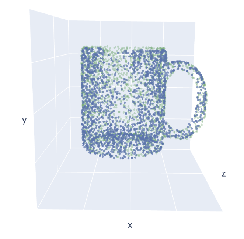
\includegraphics[width=0.3\linewidth]{imagen_rotura_real} &
    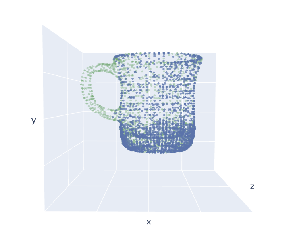
\includegraphics[width=0.3\linewidth, trim=0 0 40 0, clip]{imagen_rotura_sintetica_sn} \\
    \small Rotura real (Fantastic Breaks) &
    \small Rotura sintética (ShapeNet) \\
  \end{tabular}
  \caption{Comparativa entre una rotura real de Fantastic Breaks y una
  rotura sintética de ShapeNet (en verde, la nube completa
  (\textit{ground truth}); en azul, el fragmento roto.)}
  \label{fig:roturas_comp}
\end{figure}

Tanto las roturas sintéticas como las reales de Fantastic Breaks se llevan finalmente a
un formato común: nubes de 2.048 puntos XYZ, centradas en el origen y escaladas al
percentil 99 de la distancia al centro en lugar de a la distancia máxima, para evitar
que un único punto atípico distorsione la escala de toda la nube. Todos los pares se
guardan como ficheros \texttt{.npy}, de modo que el \textit{data loader} los trata por
igual sin distinguir su origen. Fantastic Breaks requirió además una alineación previa
con ICP entre fragmento y modelo completo, como se detalla en la
Sección~\ref{sec:datos_origen}.

% ── 6.4 ─────────────────────────────────────────────────────────────────────
\section{Baseline: PCN}
\label{sec:pcn}

La arquitectura de PCN, así como la adaptación de su resolución de salida, se describen
en la Sección~\ref{subsec:pcn_modelo}. En lugar de implementar la arquitectura desde
cero, se partió de una implementación de código abierto ya existente en PyTorch
(repositorio \texttt{qinglew/PCN-PyTorch} en GitHub), adaptándola a la resolución y al
formato de datos empleados en este trabajo.

\subsection{Experimentos y resultados}
\label{subsec:pcn_exp}

El baseline se entrenó de forma incremental (v1 a v5), como se puede ver en la Tabla \ref{tab:pcn_inic} corrigiendo en cada iteración un
problema detectado en la anterior, siempre sobre el mismo conjunto combinado de datos:
los pares reales de Fantastic Breaks y el total de roturas sintéticas generadas
(Sección~\ref{sec:datos_e3}). El primer entrenamiento (v1, 100 épocas) sirvió como
punto de partida y dio un resultado pobre (CD-L1~$=0{,}0766$); al comprobar que el error
seguía bajando al final del entrenamiento sin haberse estabilizado, se decidió alargarlo
a 400 épocas (v3), lo que ya mejoró el resultado de forma notable. Sobre esa base, en v4
se introdujo un filtro de \textit{outliers} sobre las nubes de entrada (para descartar
puntos aislados que distorsionan el centrado y la escala) y se dio más peso, dentro de
la función de pérdida, al error cometido en la nube gruesa que PCN genera como paso
intermedio (Sección~\ref{subsec:pcn_modelo}), obligando así al modelo a acertar primero
la forma general del objeto antes de refinar el detalle.

\begin{table}[H]
  \centering
  \begin{threeparttable}
  \begin{tabular}{lp{7cm}cc}
    \toprule
    Versión & Cambios & CD-L1 & F-Score \\
    \midrule
    v1 & Primer entrenamiento, 100 épocas                          & 0,0766 & 0,019 \\
    v3 & 400 épocas                                                & 0,0665 & 0,024 \\
    v4 & Filtro \textit{outliers}, más peso rama \textit{coarse}   & 0,0641 & 0,024 \\
    v5 & Corrección desalineación de centroide                    & \textbf{0,0630} & \textbf{0,026} \\
    \bottomrule
  \end{tabular}
  \begin{tablenotes}\footnotesize
    \item V2 no aparece ya que fue un intento con bug en la pérdida, detectado y descartado antes de completarse.
  \end{tablenotes}
  \caption{Experimentos del baseline PCN.}
  \label{tab:pcn_inic}
  \end{threeparttable}
\end{table}

Por último, el cambio más relevante fue el de v4 a v5: se activó una corrección en el código de
preprocesado que recentra cada par por el centroide del fragmento antes de pasarlo a la
red. Sin esta corrección, el desplazamiento de $\approx0{,}4$ unidades entre el
centroide del fragmento y el origen del objeto completo hace que el modelo colapse a
una placa plana (CD~$\approx 0{,}18$--$0{,}23$). Este principio se mantuvo en todos los
experimentos posteriores.

Aun así, v5 alcanza F-Score~$= 0{,}026$, lejos de resultados aceptables. Para averiguar
si el problema estaba en los datos o en el propio decoder, se entrenó el modelo hasta
memorizar perfectamente un único ejemplo real, sin preocuparse de que generalizara al
resto: si un modelo no es capaz ni siquiera de reproducir con precisión un solo caso
cuando se le fuerza a ello, la limitación no puede deberse a la variedad o calidad de
los datos de entrenamiento, sino a que el propio decoder no tiene capacidad suficiente
para representar bien la forma, como confirmó el resultado del experimento. Esto motivó
la exploración con TopNet.

\begin{figure}[H]
  \centering
  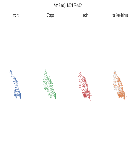
\includegraphics[width=0.8\linewidth]{pcn_muestra1}
  \caption{Mejor caso del test de PCN (CD$=0{,}0275$, F-Score$=0{,}097$). En orden: entrada rota, \textit{ground truth}, predicción del modelo y superposición de ambas.}
  \label{fig:pcn_mejor}
\end{figure}

% ── 6.5 ─────────────────────────────────────────────────────────────────────
\section{Exploración con TopNet}
\label{sec:topnet}


La arquitectura de TopNet se describe en la Sección~\ref{subsec:topnet_modelo}.
A diferencia de PCN, no se partió de una implementación externa, sino que se programó
desde cero en PyTorch puro, sin extensiones CUDA, ya que al usar una implementación de
terceros se podrían introducir diferencias de rendimiento ajenas al propio cambio de
arquitectura. Al compartir además el mismo \textit{encoder} que PCN, cualquier
diferencia de resultado entre ambos modelos es atribuible específicamente al cambio de
\textit{decoder}. El árbol implementado tiene $\approx$\,1,25\,M de parámetros
entrenables.

\subsection{Experimentos y resultados}
\label{subsec:topnet_exp}

A diferencia del baseline de PCN, TopNet no se sometió a un proceso iterativo de
varias versiones: al tratarse de un experimento dirigido específicamente a contrastar
si el decoder era el factor limitante, bastaba con una única ejecución, configurada de
forma equivalente a la mejor versión de PCN, para obtener una comparación válida.
Así, TopNet se entrenó con la misma mezcla de datos y el mismo \textit{fix} de
centroide que PCN~v5, de modo que cualquier diferencia de resultado entre ambos fuera
atribuible exclusivamente al cambio de decoder.

\begin{table}[H]
  \centering
  \begin{tabular}{lcc}
    \toprule
    Modelo & CD-L1  & F-Score  \\
    \midrule
    PCN v5  & 0,0630 & 0,0257 \\
    TopNet  & 0,0601 & 0,0329 \\
    \bottomrule
  \end{tabular}
  \caption{Comparativa PCN vs.\ TopNet.}
  \label{tab:topnet}
\end{table}

TopNet mejora a PCN en ambas métricas, y lo hace además con aproximadamente una cuarta
parte de los parámetros de PCN (Sección~\ref{sec:pcn}), lo que confirma que el
\textit{decoder} tipo \textit{folding} de PCN era, al menos parcialmente, un factor
limitante: sustituir únicamente esa pieza, sin tocar el \textit{encoder}, ya produce
una reconstrucción más ajustada con menos capacidad de red.

Aun así, la mejora sigue siendo moderada (F-Score $= 0{,}033$) y no cierra la brecha
necesaria para obtener reconstrucciones de calidad aceptable. Estos resultados
motivaron la exploración de PoinTr, que sustituye tanto el \textit{encoder} como el
\textit{decoder} por un mecanismo de atención entre puntos.

\begin{figure}[H]
  \centering
  \includegraphics[width=0.8\linewidth]{topnet_muestra1}
  \caption{Mejor caso del test de TopNet (CD$=0{,}0281$, F-Score$=0{,}271$). En orden:
           entrada rota, \textit{ground truth}, predicción del modelo y superposición
           de ambas.}
  \label{fig:topnet_mejor}
\end{figure}
% ── 6.6 ─────────────────────────────────────────────────────────────────────
\section{Modelo principal: PoinTr}
\label{sec:pointr}


La arquitectura de PoinTr, con $\approx$\,42,2\,M de parámetros entrenables, se
describe en la Sección~\ref{subsec:pointr_modelo}. Es un salto de escala considerable
respecto a los dos modelos anteriores (8 veces más parámetros que PCN y 34 veces más
que TopNet), siendo la arquitectura más compleja de las tres exploradas en
esta fase. Se usó la implementación oficial del modelo (repositorio
\texttt{yuxumin/PoinTr} en GitHub).

\subsection{Experimentos y evolución de resultados}
\label{subsec:pointr_exp}

Como ya se ha mencionado, generar las roturas sintéticas desplaza el centroide del fragmento hasta $\approx0{,}4$ unidades del origen del objeto completo, lo que sin
corrección hace que el modelo colapse a una placa plana en los peores casos (CD~$\approx 0{,}18$--$0{,}23$). Esta corrección (centrar el fragmento en su propio
centroide y desplazar el \textit{ground truth} al mismo sistema de referencia) se introdujo ya en los primeros experimentos de PoinTr y se mantuvo en todos los posteriores.

PoinTr se entrenó en seis versiones, como se puede ver en la tabla \ref{tab:pointr}. Los primeros intentos se descartaron porque parte de las mallas empleadas tenían geometrías sin
sentido que generaban ruido en el entrenamiento, lo que además hacía que la corrección
de centroide aumentara artificialmente el F-Score obtenido, sin que
fuera comparable con el resto de experimentos. Esto llevó a una nueva pasada de
limpieza de los datos, descartando de nuevo las formas en base a sus geometrías. Ya con datos limpios y bien alineados, el punto de
partida (v4) se entrenó solo con los 61 pares reales de Fantastic Breaks
(CD$=0{,}0569$).
Para ampliar el entrenamiento se probaron dos vías en paralelo: combinar esos pares
reales con Objaverse (v5\_fb\_obj) o usar solo Objaverse (v5\_obj). Pese a tener menos pares, la prueba sin datos reales obtuvo mejor resultado
(CD$=0{,}0306$ frente a $0{,}0323$), una primera señal de que mezclar pocos pares
reales con muchos sintéticos no ayudaba.

Sobre esa base sin Fantastic Breaks se añadió también ShapeNet (v6\_obj\_sn, CD$=0{,}0245$) obteniendo el mejor resultado del proyecto, sin
que se modificara la arquitectura ni los hiperparámetros respecto a v4, por lo que la mejora
vino solo de entrenar con más pares limpios y bien alineados. Al volver a añadir los
61 pares de Fantastic Breaks a este mejor modelo (v6\_fb\_obj\_sn), el
resultado empeoró (CD de 0,0245 a 0,0297, un 21\,\% peor), confirmando que con pocos pares reales frente a miles de
sintéticos uniformes, los reales pesan tan poco que actúan como ruido. Esto es
relevante para la integración final: al recibir nubes reales de fotos de objetos
rotos, el rendimiento del modelo podría ser peor que el observado aquí sobre el test
sintético.
\begin{table}[H]
  \centering
  \begin{threeparttable}
  \begin{tabular}{llcc}
    \toprule
    Versión & Datos & CD-L1 & F-Score \\
    \midrule
    v2      & Fantastic Breaks + roturas sintéticas (sin limpiar) \  & 0,0533 & 0,328 \\
    v4          & Fantastic Breaks              & 0,0569 & 0,029 \\
    v5\_fb\_obj & Fantastic Breaks + Objaverse  & 0,0323 & 0,255 \\
    v5\_obj     & Objaverse                    & 0,0306 & 0,270 \\
    v6\_fb\_obj\_sn & FB + Objaverse + ShapeNet & 0,0297 & 0,387 \\
    v6\_obj\_sn & Objaverse + ShapeNet        & \textbf{0,0245} & \textbf{0,4547} \\
    \bottomrule
  \end{tabular}
  \begin{tablenotes}\footnotesize
    \item v2 se entrenó sobre datos aún sin limpiar; la corrección de centroide
    infló artificialmente su F-Score, por lo que no es comparable con el resto de
    versiones.
  \end{tablenotes}
  \caption{Experimentos de PoinTr. Mejor resultado en \textbf{negrita}.}
  \label{tab:pointr}
  \end{threeparttable}
\end{table}


\subsection{Análisis del mejor modelo (v6\_obj\_sn)}
\label{subsec:mejor_modelo}

El modelo v6\_obj\_sn se entrenó con Objaverse y ShapeNet durante 500 épocas.
El mejor \textit{checkpoint} se alcanzó en la época 486 de 500, con la pérdida
de validación todavía descendiendo levemente.
Los resultados globales sobre el test set (251 muestras independientes) son
CD-L1~$= 0{,}0245$ y F-Score~$= 0{,}4547$.

El análisis detallado por objeto se recoge en la Tabla~\ref{tab:analisis_objeto}
del Anexo~\ref{ap:tablas}.
Entre el 78\,\% y el 92\,\% de los puntos predichos caen dentro del umbral de corrección
de~0,05 unidades normalizadas.
Los objetos de ShapeNet producen mejores resultados que los de Objaverse,
lo que refleja que ShapeNet tiene mallas más uniformes y regularmente muestreadas.

Los 6 mejores objetos del test set por CD-L1 se recogen en la
Tabla~\ref{tab:top6} del Anexo~\ref{ap:tablas}. Un ejemplo representativo se puede ver en la Figura
\ref{fig:pointr_mejor1}.

\begin{figure}[H]
  \centering
\includegraphics[width=0.9\linewidth]{imagenes/000_objaverse_9770e5a091e94eee9636b5284f8d3e4f_r0_cd0.0090.png}
  \caption{CD$=0{,}0090$, F$=0{,}679$}
  \label{fig:pointr_mejor1}
\end{figure}

% \begin{figure}[H]
%   \centering
%   \includegraphics[width=0.85\linewidth]{imagenes/001_shapenet_2927d6c8438f6e24fe6460d8d9bd16c6_cd0.0088.png}
%   \caption{CD$=0{,}0088$, F$=0{,}779$}
%   \label{fig:pointr_mejor2}
% \end{figure}

% \begin{figure}[H]
%   \centering
%   \includegraphics[width=0.85\linewidth]{imagenes/002_objaverse_9770e5a091e94eee9636b5284f8d3e4f_r2_cd0.0114.png}
%   \caption{CD$=0{,}0114$, F$=0{,}673$}
%   \label{fig:pointr_mejor3}
% \end{figure}

% \begin{figure}[H]
%   \centering
%   \includegraphics[width=0.85\linewidth]{imagenes/003_shapenet_c7fa54dc356f039d2f2318fdd66be40a_cd0.0108.png}
%   \caption{CD$=0{,}0108$, F$=0{,}575$}
%   \label{fig:pointr_mejor4}
% \end{figure}


% ── 6.7 ─────────────────────────────────────────────────────────────────────
\section{Comparativa global de arquitecturas}
\label{sec:comparativa}

\begin{table}[H]
  \centering
  \label{tab:comparativa_arq}
  \resizebox{\textwidth}{!}{%
  \begin{tabular}{lcccccc}
    \toprule
    Modelo & Params. & Encoder & Decoder & CD-L1  & F-Score & Mejor época \\
    \midrule
    PCN v5        & $\sim$5,16\,M  & PointNet MLP & FoldingNet 2D   & 0,0630 & 0,0257  & 445/500 \\
    TopNet        & $\sim$1,25\,M  & PointNet MLP & Árbol jerárquico & 0,0601 & 0,0329   & 476/500     \\
    \textbf{PoinTr v6\_obj\_sn} & \textbf{42,2\,M} & \textbf{DGCNN + atención} &
      \textbf{Transformer + FoldingNet local} & \textbf{0,0245} & \textbf{0,4547} & \textbf{486/500} \\
    \bottomrule
  \end{tabular}%
  }
  \caption{Comparativa final entre las tres arquitecturas evaluadas.}
\end{table}

La sustitución del \textit{decoder} de PCN por un árbol jerárquico (TopNet) produjo
una mejora moderada en ambas métricas; CD pasó de $0{,}063$ a $0{,}060$ y 
F-Score de $0{,}026$ a $0{,}033$, lo que confirmó que el \textit{decoder folding}
de PCN generaba peores resultados. Sin embargo, la representación global
de 1.024 dimensiones generada por PointNet resultó insuficiente para capturar la
geometría local necesaria en la tarea de \textit{shape completion}.

El salto cualitativo se produjo al reemplazar también el \textit{encoder} por una
arquitectura basada en atención (DGCNN + Transformer): en vez de resumir toda la nube
en un único vector global, cada grupo de puntos puede compararse con el resto para
decidir cómo completar la zona rota (Sección~\ref{subsec:pointr_modelo}). PoinTr
redujo el CD un 59\,\% respecto a TopNet y multiplicó el F-Score por un factor de 14,
lo que demuestra que el cuello de botella más determinante residía en el
\textit{encoder} y que las arquitecturas \textit{transformer} superan claramente a los
enfoques basados en PointNet para este tipo de tarea.

En consecuencia, se seleccionó PoinTr v6\_obj\_sn como modelo final,
empleado tanto para la generación del STL imprimible (Capítulo~\ref{ch:malla}) como en
producción con las nubes de puntos reales obtenidas a partir del modelo seleccionado
de Pix2Vox++.

\begin{figure}[H]
  \centering
  
\includegraphics[width=\linewidth]{figura_experimentos_e3}
  \caption{Evolución de CD-L1 y F-Score a lo largo de todos los experimentos de esta fase. PCN
           (v1--v5) y TopNet se entrenaron sobre el mismo conjunto de datos
           (Fantastic Breaks + roturas sintéticas); el número de pares de cada versión
           de PoinTr (versiones tras limpieza geométrica) se indica bajo cada barra.}
  \label{fig:evolucion_e3}
\end{figure}
% ============================================================
\chapter{Generación de malla imprimible}
\label{ch:malla}

\section{Formato de entrada}
\label{sec:formato_e4}


La nube de puntos que recibe esta fase no es exactamente la nube completa que produce
PoinTr (Capítulo~\ref{ch:generativo}), sino una versión algo más densa: PoinTr genera
internamente una predicción de 2.048 puntos para la región faltante, que se concatena
con la nube parcial de entrada para formar la nube completa final. Sobre ella se aplica
además un filtro de puntos atípicos, que descarta aquellos cuya distancia media a sus
puntos más próximos se aleja notablemente del resto de la nube, típicamente, errores
puntuales de la predicción. Tras este filtrado, el resultado tiene entre 3.700 y
3.900 puntos en total.

Esta densidad mayor que la nube base ayuda a cubrir mejor la superficie del objeto en
los pasos siguientes, aunque, como se verá en la Sección~\ref{sec:resultados_e4}, sigue
sin ser suficiente para generar una malla completamente cerrada.
% ── 7.2 ─────────────────────────────────────────────────────────────────────
\section{Pipeline de conversión: nube de puntos a STL}
\label{sec:pipeline_stl}

Una impresora 3D necesita una superficie cerrada, no puntos sueltos, así que la nube se
convierte en malla mediante la reconstrucción de
Poisson, que ajusta una superficie continua a la nube de
puntos. Un parámetro de este método, la profundidad, controla el
nivel de detalle que intenta capturar: cuanto más alta, más fielmente sigue los
pequeños detalles, pero también más rellena de forma arbitraria las zonas sin puntos
suficientes.

Esto último es justo lo que ocurría al aplicar Poisson directamente sobre la nube
filtrada con una profundidad alta: la malla podía superar la comprobación de
\textit{watertight} (que solo exige que la superficie esté cerrada, sin huecos), pero
con cavidades internas inventadas, sin relación con la forma real del objeto, algo que
delata el número de Euler, una medida independiente de la topología que, si se aleja
mucho del valor esperado, revela que el interior de la malla no es correcto aunque no
haya huecos visibles.

Para reducir este problema, antes de aplicar Poisson se suaviza la nube (cada punto se
desplaza levemente hacia la posición media de sus puntos más próximos, repitiendo el
proceso varias veces), atenuando el ruido disperso de PoinTr sin añadir puntos nuevos.
Sobre esta nube suavizada se intenta primero un método más conservador, el
\textit{Ball Pivoting Algorithm}, que solo genera superficie donde hay puntos
suficientes para apoyarla, dejando sin cerrar el resto en vez de inventar geometría.
En la práctica, la densidad disponible no basta para que este método funcione, así que
se recurre a Poisson con una profundidad baja: una malla más basta, pero con mucho
menos relleno inventado.

Por último, como el modelo trabaja en unidades normalizadas, cada malla se centra en
el origen y se escala para que su dimensión mayor mida 100\,mm, el tamaño de impresión
objetivo.

% ── 7.3 ─────────────────────────────────────────────────────────────────────
\section{Reparación topológica}
\label{sec:reparacion}

La malla resultante no siempre es imprimible, ya que puede arrastrar defectos propios
de este tipo de reconstrucción: \textit{aristas no-manifold} (bordes compartidos por
más de dos triángulos, o por ninguno, algo imposible en un objeto físico real), huecos,
caras mal orientadas y fragmentos desconectados del resto (normalmente restos de la
reconstrucción en zonas con pocos puntos de referencia), precisamente donde Poisson
tiene menos información real sobre la que apoyarse.

Para corregirlos se aplica una cadena de reparación en varios pasos, cada uno pensado
para resolver lo que el anterior no consiga. Primero se descartan los fragmentos
sueltos, quedándose solo con el de mayor tamaño. Sobre esa malla se intenta una
reconstrucción topológicamente correcta con
ManifoldPlus, que reconstruye la superficie de forma que
cada arista quede compartida exactamente por dos caras. Si falla, se recurre a
pymeshlab: se eliminan caras duplicadas o degeneradas, se reparan directamente las
aristas y vértices problemáticos, y se cierran los huecos en tres pasadas de dificultad
creciente (hasta 30, 150 y 500 aristas). Por último se aplica un cierre de huecos
residuales y se corrige la orientación de los triángulos hacia el exterior.

Pese a esta cadena, como se muestra en la Sección~\ref{sec:resultados_e4}, no todos los
defectos se corrigen del todo: el proceso mejora la malla de forma clara, pero no logra una superficie completamente cerrada.
% ── 7.4 ─────────────────────────────────────────────────────────────────────
\section{Validación para impresión 3D}
\label{sec:validacion}

Una vez reparada, cada malla se somete a una validación automática. Los criterios
empleados se recogen en la Tabla~\ref{tab:validacion}.

\begin{table}[H]
  \centering
  \begin{threeparttable}
  \begin{tabularx}{\linewidth}{lX}
    \toprule
    Criterio & Descripción \\
    \midrule
    \textit{Watertight} &
      La malla no tiene ningún hueco: toda arista está compartida por exactamente
      dos triángulos. \\
    Volumen positivo$^*$ &
      La malla encierra un volumen real, con las caras orientadas hacia fuera. \\
    Mínimo de caras ($\geq 100$) &
      Descarta mallas degeneradas que hubieran colapsado durante la reparación. \\
    Número de Euler $= 2$ &
      Indica una topología cerrada simple (sin agujeros que la atraviesen).
      Un objeto con asa tiene Euler~$= 0$ y también es perfectamente imprimible. \\
    \bottomrule
  \end{tabularx}
  \begin{tablenotes}\footnotesize
    \item[$*$] Solo puede calcularse un volumen fiable sobre una malla \textit{watertight};
    si la malla tiene huecos, este criterio falla automáticamente junto con el anterior.
  \end{tablenotes}
  \caption{Criterios de validación automática de la malla para impresión 3D.}
  \label{tab:validacion}
  \end{threeparttable}
\end{table}

El número de Euler es una forma de contar, a partir del número de vértices, aristas y
caras de la malla, cuántos agujeros pasantes tiene su superficie, independientemente de su forma concreta: un objeto sin ningún agujero de este
tipo (como una taza sin asa) tiene Euler~$=2$; uno con un único agujero
pasante (como una taza con asa) tiene Euler~$=0$. Por eso este criterio es
solo informativo y no bloquea la validación: ambos casos son perfectamente
imprimibles, y lo único que indica un valor alejado de estos dos números es que algo en
la topología de la malla no es correcto.
% ── 7.5 ─────────────────────────────────────────────────────────────────────
\section{Resultados y limitaciones}
\label{sec:resultados_e4}

El pipeline se puso a prueba de dos formas distintas, y ambas llegaron a la misma
conclusión. Primero, se tomaron mallas ya generadas por Poisson y se les aplicó
únicamente la reparación topológica (Sección~\ref{sec:reparacion}), para comprobar si
ese paso bastaba por sí solo: ninguna resultó \textit{watertight}, y en la mayoría de
los casos el número de Euler quedó incluso más alejado del valor esperado que antes de
reparar. Después, se probó el pipeline completo (Sección~\ref{sec:pipeline_stl}, desde
la nube de puntos hasta la malla reparada) sobre los objetos de mejor reconstrucción del
test set: de nuevo, ninguna malla resultó \textit{watertight}
(Tabla~\ref{tab:resultados_e4} del Anexo~\ref{ap:tablas}), pese a tratarse de algunas de
las reconstrucciones más fieles de PoinTr (CD medio de 0,0214, frente a 0,0408 en todo
el test set) y con formas reconocibles en todos los casos.

Para descartar que el problema viniera de errores de PoinTr, se repitió el mismo
pipeline sustituyendo la nube predicha por la nube \textit{ground truth} real de cada
objeto, sin ningún error de reconstrucción. Tampoco así se obtuvo ninguna malla
\textit{watertight} (Tabla~\ref{tab:control_gt} del Anexo~\ref{ap:tablas}), lo que
confirma que la causa no está en lo que predice PoinTr, sino en la densidad de puntos:
con solo unos miles de puntos repartidos sobre la superficie del objeto, quedan huecos
que Poisson solo puede cerrar inventando geometría interna.

\begin{figure}[H]
  \centering
  \begin{tabular}{cc}
    \includegraphics[width=0.46\linewidth]{imagenes/newplot (3).png} &
    \includegraphics[width=0.46\linewidth]{imagenes/newplot (2).png} \\
  \end{tabular}

  \vspace{1em}

  \begin{tabular}{cc}
    \includegraphics[width=0.46\linewidth]{imagenes/newplot (1).png} &
    \includegraphics[width=0.46\linewidth]{imagenes/newplot.png} \\
  \end{tabular}
  \caption{Ejemplo ilustrativo del problema de densidad: arriba, la nube de puntos
           completa
           vista desde dos ángulos; abajo, la malla resultante tras aplicar Poisson}
  \label{fig:ejemplo_hueco}
\end{figure}

En la práctica, ninguna malla pasa la validación \textit{watertight} estricta, pero
todas conservan una forma reconocible y son procesables por laminadores de impresión 3D
modernos (Cura, PrusaSlicer), que aplican su propia reparación automática. La
limitación de fondo es de resolución: con 2.048 puntos base, zonas como asas, bordes
finos o concavidades profundas no tienen densidad suficiente para que Poisson las
reconstruya con fidelidad. Aumentar la resolución de salida de PoinTr a 4.096 puntos o
más reduciría este problema de forma directa.
% ============================================================
\chapter{Conclusiones}
\label{ch:conclusiones}

\section{Limitaciones}
\label{sec:limitaciones}

El \textit{fine-tuning} sobre geometrías rotas mejora de forma notable la capacidad del
modelo (IoU medio de~0,055 a~0,311), pero el resultado sigue siendo parcial: un Dice
de~0,45 indica que la reconstrucción capta la forma general de la fractura sin ajustarse
con precisión a sus bordes, y la dispersión entre objetos es alta, 25 de las 26 tazas
de test mejoran, pero la magnitud de la mejora varía de $+0{,}03$ a $+0{,}62$ de IoU,
lo que sugiere que el modelo generaliza de forma desigual según la severidad y orientación
del corte.

Dos factores del propio diseño experimental limitan hasta dónde puede llegar esta
adaptación.
Primero, las roturas de entrenamiento y validación (532 variantes) se generaron
sintéticamente mediante cortes planos aleatorios sobre las mismas 172 mallas de partida:
el modelo aprende a reconstruir muchas variantes de fractura, pero siempre sobre la misma
base geométrica limitada.
Segundo, un corte por plano produce un borde de fractura recto y regular, muy distinto de
la geometría irregular y multiaxial de una rotura física real, por lo que no está
garantizado que el rendimiento observado se mantenga sobre fracturas reales.

Existe además una pérdida de detalle geométrico en la propia cadena del pipeline,
independiente de la calidad de las predicciones de cada modelo. La salida de
Pix2Vox++ es una rejilla de vóxeles de resolución $32^3$, por lo que, al convertirla en
nube de puntos (Sección~\ref{sec:motivacion_generativo}), las coordenadas resultantes
solo pueden ocupar posiciones múltiplos de $1/32\approx 0{,}031$ unidades. En objetos
con geometría fina, como asas o bordes delgados, esto puede perder detalle que el
modelo de reconstrucción había capturado implícitamente, antes incluso de que la nube
llegue al modelo generativo. Esta pérdida se suma a la limitación de densidad ya
identificada en la generación de la malla final (Sección~\ref{sec:resultados_e4}): el
pipeline pierde resolución tanto a la entrada de la fase de completado (por la rejilla
de vóxeles) como a la salida (por el número de puntos generados).

\section{Trabajo futuro}
\label{sec:trabajo_futuro}

A lo largo del desarrollo del proyecto han surgido diversas líneas de mejora que
no han podido abordarse en el alcance del presente trabajo pero que representan
continuaciones naturales del mismo.

En lo que respecta a la calidad de las reconstrucciones, resulta de interés
aumentar tanto la resolución de la rejilla de vóxeles de Pix2Vox++ para
reducir la cuantización en la conversión a nube de puntos y preservar el detalle
fino, como la resolución de salida de PoinTr a 4.096 o más puntos, lo que
mejoraría la densidad de la nube entregada a la fase de generación de malla y,
con ello, la calidad del STL final.

Respecto al entrenamiento, sería valioso incorporar datos de Fantastic Breaks de
forma ponderada o mediante técnicas de \textit{domain adaptation}, con el fin de
reducir la brecha entre las nubes sintéticas empleadas durante el entrenamiento y
las nubes reales obtenidas del modelo de reconstrucción. En la misma línea,
continuar explorando el doble entrenamiento, ampliando el número de imágenes,
generando nuevas roturas sintéticas o aplicando \textit{fine-tuning} adicional,
podría reportar mejoras significativas en el rendimiento del sistema.

En cuanto a la generalización del pipeline, se plantea ampliar el conjunto de
categorías más allá de las vasijas para evaluar su comportamiento con otros tipos
de objetos, así como explorar variantes de reconstrucción de superficie como
\textit{Neural Implicit Functions} o métodos basados en campos de distancia
signada, que no dependan de la densidad de la nube de entrada. Asimismo, el
pipeline podría adaptarse al conjunto de datos propio de cualquier sector
interesado en aplicarlo, como patrimonio cultural, manufactura o medicina,
facilitando su transferencia a casos de uso reales.

Por último, se contempla continuar el desarrollo de la aplicación web integrada,
actualmente en fase de prototipo funcional, que unifica todas las etapas del
pipeline en una interfaz accesible, con el objetivo de alcanzar un despliegue
estable en producción (véase \hyperref[anexo:app]{Anexo~C}).

% ============================================================
% ── ANEXO ────────────────────────────────────────────────────────────────────
% ============================================================
\clearpage
\appendix
\titleformat{\chapter}[hang]
  {\Large\bfseries}{Anexo \thechapter:}{0.7em}{}
\chapter{Tablas de resultados}
\label{ap:tablas}


Las tablas de este anexo recogen los resultados numéricos completos del proyecto, cuyo tamaño impediría una lectura cómoda en el cuerpo principal del documento.



\begin{table}[H]
  \centering
  \resizebox{\textwidth}{!}{%
  \begin{tabular}{clccccccccccc}
    \toprule
    Num.\ Exp. & Tipo Experimento & Modelo & N categorías & Vistas & N test & Umbral & IoU & Dice & Precisión voxel & Recall voxel & Chamfer & F-score \\
    \midrule
    1 & tazas\_1\_vista\_sin\_finetuning    & ResNet-50 & 1 & 1  & 26 & 0,2 & 0,17  & 0,2823 & 0,3167 & 0,309  & 2,4174 & 0,3594 \\
    2 & tazas\_5\_vistas\_sin\_finetuning   & ResNet-50 & 1 & 5  & 26 & 0,2 & 0,159 & 0,2606 & 0,3422 & ,2367 & 2,6474 & 0,3097 \\
    3 & tazas\_20\_vistas\_sin\_finetuning  & ResNet-50 & 1 & 20 & 26 & 0,2 & 0,158 & 0,2608 & 0,3337 & 0,2434 & 2,7197 & 0,3016 \\
    4 & tazas\_1\_vista\_con\_finetuning    & ResNet-50 & 1 & 1  & 26 & 0,2 & 0,398 & 0,5544 & 0,4285 & 0,8755 & 1,3218 & 0,6199 \\
    5 & tazas\_5\_vistas\_con\_finetuning   & ResNet-50 & 1 & 5  & 26 & 0,2 & 0,534 & 0,6815 & 0,5993 & 0,8199 & 0,8572 & 0,8016 \\
    6 & tazas\_20\_vistas\_con\_finetuning  & ResNet-50 & 1 & 20 & 26 & 0,2 & 0,558 & 0,6968 & 0,647  & 0,7826 & 0,8036 & 0,8121 \\
    \bottomrule
  \end{tabular}%
  }
  \caption{Resultados de los experimentos 1-6 (sin y con \textit{fine-tuning}), para tazas con 1, 5 y 20 vistas}
  \label{tab:resultados_finetuning}
\end{table}


\begin{table}[H]
  \centering
  \resizebox{\textwidth}{!}{%
  \begin{tabular}{clccccccccccc}
    \toprule
    Num.\ Exp. & Tipo Experimento & Modelo & N categorías & Vistas & N test & Umbral & IoU & Dice & Precisión voxel & Recall voxel & Chamfer & F-score \\
    \midrule
    7  & tazas\_botellas\_20\_vistas\_sin\_finetuning              & ResNet-50       & 2 & 20 & 94  & 0,15 & 0,122 & 0,1977 & 0,3413 & 0,1599 & 4,1091 & 0,2042 \\
    8  & tazas\_botellas\_20\_vistas\_con\_finetuning              & ResNet-50       & 2 & 20 & 26  & 0,4  & 0,793 & 0,8655 & 0,8626 & 0,8742 & 0,3244 & 0,9395 \\
    9  & exp9\_4categorias\_20v\_finetuning\_test\_global           & ResNet-50       & 4 & 20 & 198 & 0,3  & 0,693 & 0,7977 & 0,7818 & 0,831  & 0,6137 & 0,8536 \\
    9  & exp9\_4categorias\_20v\_finetuning\_test\_tazas            & ResNet-50       & 4 & 20 & 26  & 0,3  & 0,584 & 0,7199 & 0,6991 & 0,7626 & 0,7148 & 0,8363 \\
    10 & exp10\_4categorias\_5v\_finetuning\_test\_global           & ResNet-50       & 4 & 5  & 198 & 0,3  & 0,702 & 0,8068 & 0,7775 & 0,8571 & 0,5755 & 0,8674 \\
    10 & exp10\_4categorias\_5v\_finetuning\_test\_tazas            & ResNet-50       & 4 & 5  & 26  & 0,3  & 0,592 & 0,7287 & 0,701  & 0,7821 & 0,652  & 0,8575 \\
    11 & exp11\_fix\_experimento8\_20v\_finetuning\_test\_global    & ResNet-50       & 2 & 20 & 94  & 0,3  & 0,729 & 0,8265 & 0,8272 & 0,8406 & 0,5663 & 0,8662 \\
    11 & exp11\_fix\_experimento8\_20v\_finetuning\_test\_tazas     & ResNet-50       & 2 & 20 & 26  & 0,15 & 0,568 & 0,7099 & 0,6716 & 0,7768 & 0,7191 & 0,8285 \\
    12 & exp12\_4categorias\_5v\_efficientnetb4\_finetuning\ldots   & EfficientNet-B4 & 4 & 5  & 198 & 0,3  & 0,661 & 0,7762 & 0,7223 & 0,8658 & 0,6887 & 0,8292 \\
    12 & exp12\_4categorias\_5v\_efficientnetb4\_finetuning\ldots   & EfficientNet-B4 & 4 & 5  & 26  & 0,4  & 0,547 & 0,6913 & 0,647  & 0,7755 & 0,703  & 0,8328 \\
    13 & exp13\_7categorias\_5v\_finetuning\_test\_global           & ResNet-50       & 7 & 5  & 327 & 0,3  & 0,65  & 0,7623 & 0,7289 & 0,8248 & 0,6855 & 0,8343 \\
    13 & exp13\_7categorias\_5v\_finetuning\_test\_tazas            & ResNet-50       & 7 & 5  & 26  & 0,3  & 0,606 & 0,7417 & 0,7031 & 0,8034 & 0,6236 & 0,8688 \\
    14 & exp14\_6categorias\_5v\_finetuning\_test\_global           & ResNet-50       & 6 & 5 & 253 & 0,4 & 0,7012 & 0,8039 & -- & -- & 0,5745 & 0,8677 \\
    14 & exp14\_6categorias\_5v\_finetuning\_test\_tazas            & ResNet-50       & 6 & 5  & 26  & 0,4 & 0,6005 & 0,7341 & -- & -- & 0,6399 & 0,8634 \\
    \bottomrule
  \end{tabular}%
  }
  \caption{Resultados de los experimentos 7--14 (categorías combinadas y \textit{fine-tuning}).}
  \label{tab:resultados_categorias}
\end{table}







% ── A.1 ──────────────────────────────────────────────────────────────────────
\begin{table}[H]
  \centering
  
  \label{tab:experimentos_e3}
  \begin{threeparttable}
    \resizebox{\textwidth}{!}{%
    \begin{tabular}{llllrrrcc p{4.5cm}}
      \toprule
      Versión & Modelo & Datos & Limpios & Pares & $N_{\text{test}}$ &
      Mejor ép. & CD-L1 & F-Score & Observaciones \\
      \midrule
      PCN v1             & PCN    & FB (desalineado) + sint.\ inicial        & No & 2.428 & 237 & 97  & 0,0766 & 0,019 & primer baseline \\
      PCN v3             & PCN    & FB (desalineado) + sint.\ inicial        & No & 2.428 & 237 & 347 & 0,0665 & 0,024 & 400 épocas \\
      PCN v4             & PCN    & FB (desalineado) + sint.\ (plano+chip+cuña) & No & 2.360 & 236 & 480 & 0,0641 & 0,024 & \\
      PCN v5             & PCN    & FB (desalineado) + sint.\ (plano+chip+cuña) & Centrado & 2.360 & 236 & 445 & 0,0630 & 0,026 & corrección de centroide activada; mejor PCN \\
      TopNet             & TopNet & FB (desalineado) + sint.\ (plano+chip+cuña) & Centrado & 2.360 & 131 & 476 & 0,0601 & 0,0329 & misma configuración de datos que PCN v5 \\
      PoinTr v2          & PoinTr & FB (desalineado) + sint.\ filtrado & No & 402   & 41  & 150 & 0,0533 & 0,328$^a$ & F-Score inflado; datos sin limpiar \\
      PoinTr v4          & PoinTr & Fantastic Breaks       & Sí & 61    & 7   & 285 & 0,0569 & 0,029 & primer experimento con datos limpios \\
      PoinTr v5\_fb\_obj & PoinTr & FB + Objaverse         & Sí & 458   & 47  &  ---& 0,0323 & 0,255 & primera combinación real + sintético limpio \\
      PoinTr v5\_obj     & PoinTr & Objaverse               & Sí & 397   & 41  &  ---& 0,0306 & 0,270 & sin FB; referencia antes de ShapeNet \\
      PoinTr v6\_fb\_obj\_sn & PoinTr & FB + Objaverse + ShapeNet & Sí & 2.562 & 132 &  ---& 0,0297 & 0,387 & añadir FB empeora el CD respecto a v6\_obj\_sn \\
      \textbf{PoinTr v6\_obj\_sn} & \textbf{PoinTr} & \textbf{Objaverse + ShapeNet} &
        \textbf{Sí} & \textbf{2.501} & \textbf{251} & \textbf{486/500} &
        \textbf{0,0245} & \textbf{0,4547} & \textbf{Mejor modelo del proyecto} \\
      \bottomrule
    \end{tabular}}
    \begin{tablenotes}\footnotesize
      \item $^a$ PoinTr v2: F-Score inflado por la corrección de centroide aplicada
            sobre datos aún sin limpiar, 
            no comparable con el resto.
    \end{tablenotes}
  \end{threeparttable}
  \caption{Todos los experimentos de la fase de \textit{shape completion}, ordenados
           cronológicamente dentro de cada modelo.}
\end{table}

% ── A.2 ──────────────────────────────────────────────────────────────────────
\begin{table}[H]
  \centering
  \begin{threeparttable}
    \begin{tabular}{lcccc}
      \toprule
      Objeto & CD-L1 & \% correctos ($<0{,}05$) & Puntos erróneos & GT sin cubrir \\
      \midrule
      shapenet\_14588e37\dots & 0,0177 & \textbf{92\,\%} & 311 & 344 \\
      shapenet\_fa23aa60\dots & 0,0233 & 90\,\% & 404 & 202 \\
      shapenet\_f1e43930\dots & 0,0252 & 86\,\% & 554 & 373 \\
      shapenet\_62d897a9\dots & 0,0302 & 86\,\% & 588 & 583 \\
      objaverse\_1095a05d\dots (r0) & 0,0306 & 83\,\% & 700 & 316 \\
      shapenet\_93c83723\dots & 0,0297 & 78\,\% & 896 & 375 \\
      \bottomrule
    \end{tabular}
    \begin{tablenotes}\footnotesize
      \item Punto correcto: distancia al punto de \textit{ground truth} más cercano
            $< 0{,}05$ unidades normalizadas.
    \end{tablenotes}
  \end{threeparttable}
  \caption{Análisis de algunos objetos del mejor modelo v6\_obj\_sn: puntos correctos frente a  erróneos con umbral~$t=0{,}05$.}
    \label{tab:analisis_objeto}
\end{table}

% ── A.3 ──────────────────────────────────────────────────────────────────────
\begin{table}[H]
  \centering
  \begin{threeparttable}
    \begin{tabular}{clccc}
      \toprule
      N.º & Objeto & CD-L1 & F-Score & \textit{Outliers} eliminados \\
      \midrule
      \textbf{1} & \textbf{shapenet\_c7fa54dc\dots}    & \textbf{0,0118} & \textbf{0,6249} & \textbf{166} \\
      2          & shapenet\_98d34080\dots               & 0,0124 & 0,5971 & 139 \\
      3          & objaverse\_9770e5a0\dots (r0)         & 0,0127 & 0,6259 & 241 \\
      4          & shapenet\_ee74f5bf\dots               & 0,0134 & 0,5623 & 112 \\
      5          & shapenet\_2927d6c8\dots               & 0,0155 & 0,7436 & 299 \\
      6          & shapenet\_3dbd6642\dots               & 0,0162 & 0,5577 & 338 \\
      \bottomrule
    \end{tabular}
    \begin{tablenotes}\footnotesize
      \item Resultados obtenidos sobre una partición de 126 pares, más reducida que el
            test set completo de 251 muestras usado para los resultados oficiales del
            modelo (Sección~\ref{subsec:mejor_modelo}). CD medio sobre esta partición:
            0,0408 (0,0214 restringido a estos 6 objetos). Peor objeto de la partición:
            CD$=0{,}1878$.
    \end{tablenotes}
    \caption{Los 6 objetos con menor CD-L1 de la partición usada para generar los STL
             de ejemplo.}
    \label{tab:top6}
  \end{threeparttable}
\end{table}

% ── A.4 ──────────────────────────────────────────────────────────────────────
\begin{table}[H]
  \centering
  \begin{threeparttable}
    \begin{tabular}{clcclrcc}
      \toprule
      N.º & Objeto & CD-L1 & F-Score & Método & Caras & \textit{Watertight} & Euler \\
      \midrule
      1 & shapenet\_f76b14ff\dots   & 0,0184 & 0,4849 & Poisson $d{=}7$+suav. & 32.503 & No & $-73$ \\
      2 & objaverse\_ca4f9a92\dots  & 0,0208 & 0,5876 & Poisson $d{=}7$+suav. & 23.483 & No & $-33$ \\
      3 & shapenet\_1ae1ba5d\dots   & 0,0217 & 0,3932 & Poisson $d{=}7$+suav. & 27.713 & No & $-18$ \\
      4 & shapenet\_24f615dd\dots   & 0,0218 & 0,4993 & Poisson $d{=}7$+suav. & 26.402 & No & $-47$ \\
      5 & objaverse\_d40aa57b\dots  & 0,0227 & 0,4557 & Poisson $d{=}7$+suav. & 20.659 & No & $0$ \\
      6 & objaverse\_57be7663\dots (r1) & 0,0232 & 0,2755 & Poisson $d{=}7$+suav. & 21.666 & No & $-12$ \\
      \bottomrule
    \end{tabular}
    \begin{tablenotes}\footnotesize
      \item Pipeline aplicado: filtrado de puntos atípicos,
            suavizado Laplaciano + \textit{Ball Pivoting} +
            Poisson ($\texttt{depth}=7$) + reparación topológica. El \textit{Ball
            Pivoting} falló en los 6 casos, por lo que todos se procesaron con
            Poisson. Ninguno resultó \textit{watertight}. 
    \end{tablenotes}
    \caption{Resultados de generación de malla para los 6 objetos con menor CD-L1 de
             la Tabla~\ref{tab:top6}.}
    \label{tab:resultados_e4}
  \end{threeparttable}
\end{table}

% ── A.5 ──────────────────────────────────────────────────────────────────────
\begin{table}[H]
  \centering
  \begin{threeparttable}
    \resizebox{\textwidth}{!}{%
    \begin{tabular}{lrcrrp{5cm}}
      \toprule
      Objeto & Puntos & Caras & \textit{Watertight} & Euler & Observación \\
      \midrule
      shapenet\_c7fa54dc\dots (GT) & 2.048 & 12.376 & No & $0$    & Topología correcta (de objeto con asa), no cerrada \\
      shapenet\_98d34080\dots (GT) & 2.048 & 24.293 & No & $-42$  & Cavidades internas inventadas \\
      objaverse\_9770e5a0\dots (GT)& 2.048 & 28.491 & No & $-113$ & Euler muy alejado de 2; mucha geometría interna inventada \\
      shapenet\_ee74f5bf\dots (GT) & 2.048 &  8.716 & No & $-23$  & Componente principal de 3 fragmentos detectados \\
      shapenet\_2927d6c8\dots (GT) & 2.048 &  6.395 & No & $1$    & Geometría simple, cercana a una esfera \\
      shapenet\_3dbd6642\dots (GT) & 2.048 & 19.207 & No & $-24$  & Cavidades internas inventadas \\
      \bottomrule
    \end{tabular}}
    \begin{tablenotes}\footnotesize
      \item Ninguno de los 6 objetos resultó \textit{watertight}, pese a partir de
            nubes de \textit{ground truth} perfectas (sin error de predicción).
    \end{tablenotes}
    \caption{Experimento de control: generación de malla a partir de nubes de
             \textit{ground truth} perfectas, en lugar de las predicciones de PoinTr.}
    \label{tab:control_gt}
  \end{threeparttable}
\end{table}


% ============================================================
% ── ANEXO B — Planificación, metodología y resultados ────────────────────────
% ============================================================
\clearpage
\chapter{Planificación, metodología y resultados}
\label{ap:planificacion}

% ── B.1 Metodología ──────────────────────────────────────────────────────────
\section{Metodología de trabajo}

El proyecto adoptó un enfoque iterativo e incremental adaptado a la investigación
en aprendizaje profundo: los dos módulos de IA se desarrollaron en paralelo,
con contratos de interfaz cerrados desde el inicio que garantizaron la compatibilidad
de formatos sin necesidad de coordinación constante.

La experimentación fue sistemática y comparativa en ambos frentes.
En \textbf{reconstrucción 3D}, se diseñaron y evaluaron 13~experimentos sobre Pix2Vox++,
variando el número de vistas de entrada, la aplicación de \textit{fine-tuning} y la
composición del conjunto de categorías de entrenamiento.
En \textbf{reparación de objetos rotos}, se entrenaron y evaluaron 9~versiones de
modelos de completado de forma (PCN v1--v5, TopNet, PoinTr v1--v6), utilizando las
mismas particiones de datos y las mismas métricas (Chamfer Distance y F-Score) para
poder comparar arquitecturas de forma objetiva.

En ambos casos se descartaron las versiones que no superaban las anteriores y se
refinaron las prometedoras, siguiendo un ciclo de experimentación que priorizó la
validación empírica sobre la elección teórica.

% ── B.2 Planificación ────────────────────────────────────────────────────────
\section{Planificación --- Diagrama de Gantt}

\begin{figure}[H]
  \centering
  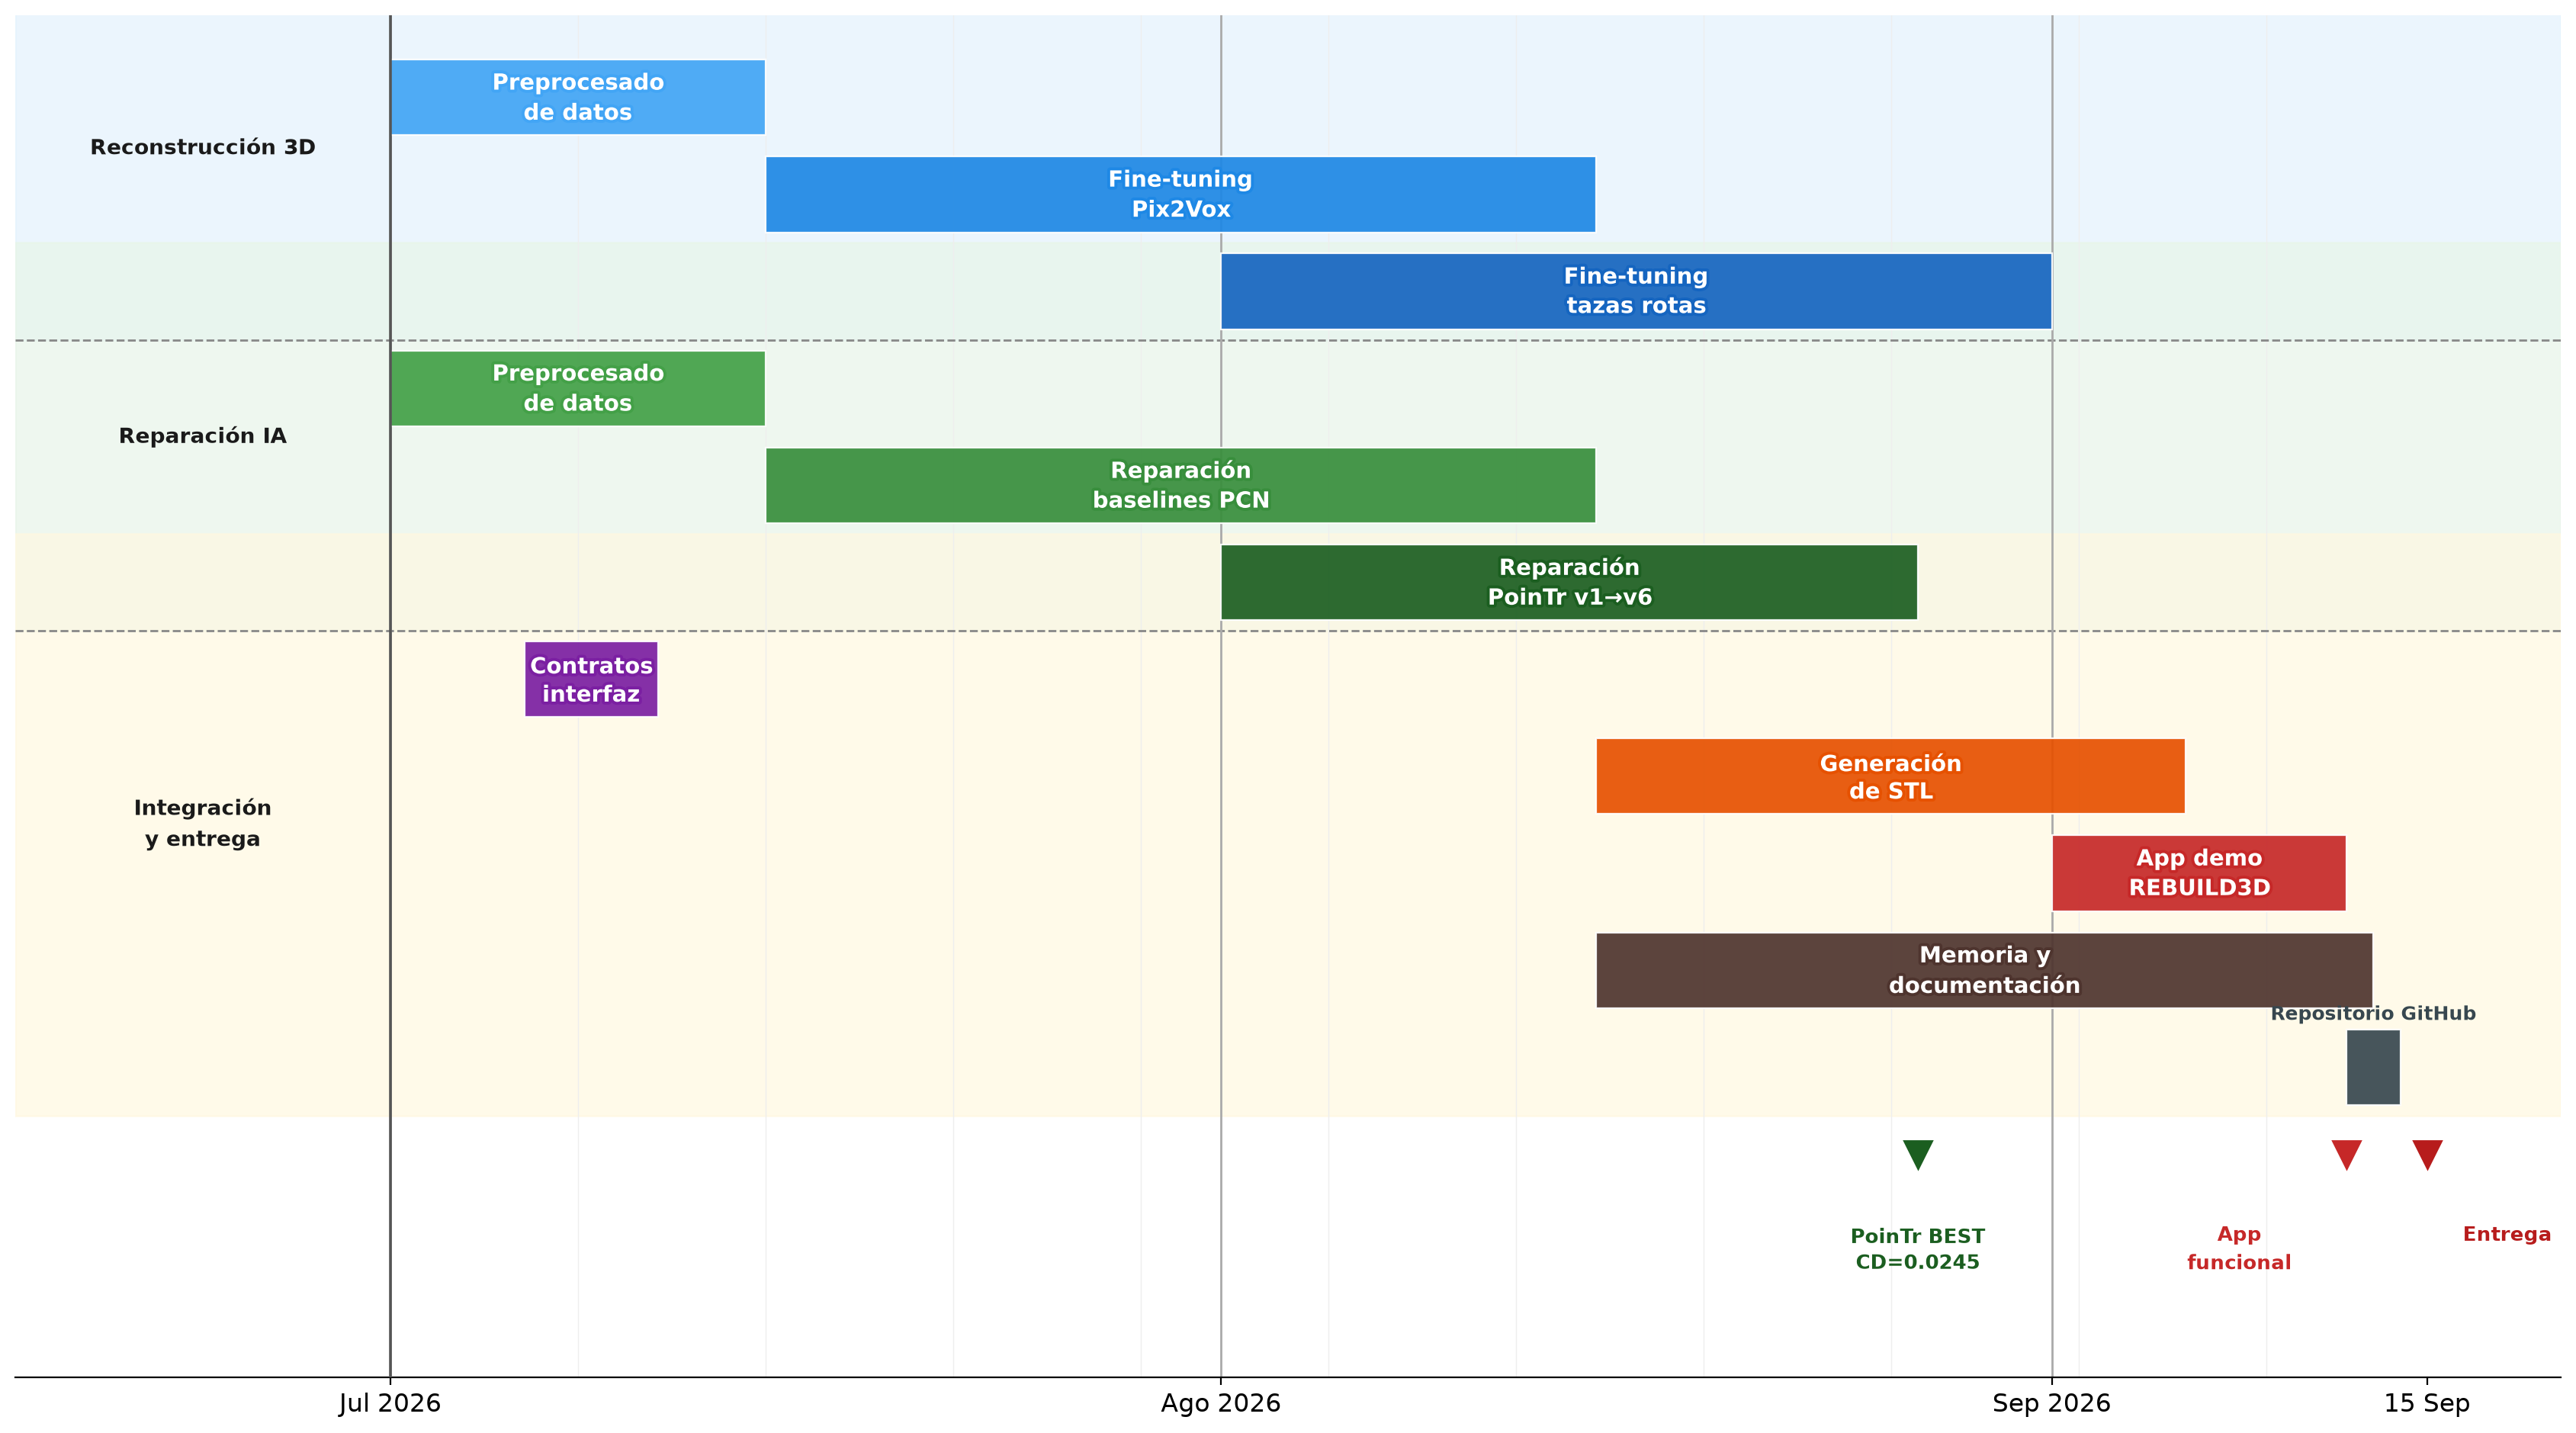
\includegraphics[width=\textwidth]{figura_gantt_anexo}
  \caption{Diagrama de Gantt del proyecto (julio--septiembre 2026).}
  \label{fig:gantt}
\end{figure}

El proyecto se estructuró en tres frentes de trabajo solapados en el tiempo.
La \textbf{reconstrucción 3D} (banda azul) abarcó la preparación de imágenes
sintéticas y el \textit{fine-tuning} de Pix2Vox++ sobre objetos completos y rotos,
generando las nubes de puntos incompletas que alimentan la siguiente fase.
La \textbf{reparación IA} (banda verde) desarrolló y validó el modelo de
completado de forma, con preprocesado de datos propio e iteraciones desde baselines
simples hasta PoinTr.
La \textbf{integración y entrega} (banda amarilla) conectó todos los módulos
en un pipeline funcional, incluyendo la generación de STL, la aplicación demo
REBUILD3D y la documentación del proyecto.

Los hitos principales fueron: contratos de interfaz cerrados (11~jul),
mejor resultado de PoinTr~v6 con CD\,=\,0{,}0245 (27~ago),
pipeline \textit{end-to-end} funcional con fotos reales (12~sep)
y entrega final (15~sep~2026).

% ── B.3 Resultados ───────────────────────────────────────────────────────────
\section{Resultados cuantificables}

\begin{table}[H]
\centering
\begin{tabular}{l p{5.5cm} p{5cm}}
\toprule
\textbf{Módulo} & \textbf{Descripción} & \textbf{Mejor resultado} \\
\midrule
Reconstrucción 3D
  & Pix2Vox++ con \textit{fine-tuning}; 13 experimentos evaluados
  & IoU\,=\,0{,}534, F-Score\,=\,0{,}802 (objetos completos, 5 vistas) \\[4pt]
Reconstrucción en rotos
  & Pix2Vox++ evaluado sobre objetos con fracturas reales y sintéticas
  & IoU mejora de 0{,}055 a 0{,}311 con \textit{fine-tuning} \\[4pt]
Reparación IA
  & Shape completion con PCN, TopNet y PoinTr; 9 versiones entrenadas
  & CD\,=\,0{,}0245, F-Score\,=\,0{,}455 (PoinTr v6\_obj\_sn) \\[4pt]
Dataset
  & ShapeNet + Objaverse + Fantastic Breaks
  & 2.562 pares nube rota / nube completa \\[4pt]
Generación de STL
  & Poisson + reparación topológica en cascada (manifold3d + pymeshlab)
  & Mallas de 6.000--32.000 caras; procesables por Cura y PrusaSlicer \\[4pt]
App demo REBUILD3D
  & Pipeline completo: fotos reales $\to$ STL imprimible (Gradio)
  & Demo funcional con tazas rotas reales \\
\bottomrule
\end{tabular}

\caption{Principales resultados obtenidos por módulo del pipeline.}
\end{table}

% ── B.4 Impacto potencial ────────────────────────────────────────────────────
\section{Impacto potencial}

La tecnología desarrollada tiene aplicación directa en tres ámbitos:

\begin{itemize}

  \item \textbf{Control de calidad industrial}: detección y modelado de la geometría
    faltante en componentes dañados, integrándose en flujos de mantenimiento
    predictivo o fabricación de piezas de recambio.

  \item \textbf{Impresión 3D bajo demanda}: cualquier usuario puede fotografiar un
    objeto roto y obtener un archivo STL listo para reimprimir la pieza dañada,
    sin conocimientos técnicos previos.
    \item \textbf{Restauración de patrimonio cultural}: reconstrucción digital de
    piezas arqueológicas o artísticas dañadas a partir de fotografías, sin necesidad
    de equipos de escaneado especializado.
\end{itemize}

% ── B.5 Riesgos ──────────────────────────────────────────────────────────────
\section{Gestión de riesgos}

\begin{table}[H]
\centering
\small
\caption{Riesgos identificados durante el proyecto, valoración y respuesta adoptada.}
\begin{tabular}{c p{3.1cm} p{1.3cm} p{1.3cm} p{5.5cm}}
\toprule
\textbf{ID} & \textbf{Riesgo} & \textbf{Prob.} & \textbf{Impacto} & \textbf{Respuesta adoptada} \\
\midrule
R1 & Cantidad de datos de entrenamiento insuficiente & Alta & Alto &
  Se combinaron tres fuentes: ShapeNet, Objaverse y Fantastic Breaks, obteniendo 2.562 pares nube rota / nube completa. \\
R2 & Muchos modelos 3D del dataset tenían geometrías inválidas: formas sin sentido, distancias extremas entre puntos o mallas no procesables & Alta & Alto &
  Limpieza manual del dataset en dos pasadas y seleccion de categorias de objetos concretas. Escalar el proceso a datasets mayores requerirá automatización. \\
R3 & Los modelos de IA no mejoraban entre iteraciones o no superaban el resultado anterior & Media & Alto &
  Se entrenaron y compararon 22 versiones (13 de Pix2Vox++, 9 de shape completion) usando siempre las mismas métricas y el mismo conjunto de test; se descartó cualquier versión que no mejorara. \\
R4 & Los modelos entrenados con datos sintéticos rinden peor al recibir nubes de puntos procedentes de fotos reales & Alta & Alto &
  Se probó incorporar los 61 pares reales de Fantastic Breaks, pero empeoró la Chamfer Distance un 21\,\%; se optó por entrenar solo con datos sintéticos y documentar la limitación como trabajo futuro. \\
R5 & Las fotos reales introducidas en la app tienen ruido y condiciones de iluminación que el pipeline no vio durante el entrenamiento & Media & Medio &
  Se implementó eliminación de fondo por umbral de luminosidad en espacio LAB (OpenCV) para reducir el ruido de entrada; limitación conocida y documentada. \\
R6 & Sin acceso a GPU de alta capacidad los tiempos de entrenamiento son inviables & Alta & Alto &
  Se contrató Google Colab Pro+ para acceder a GPUs~A100; sin este recurso, un entrenamiento de 500 épocas habría tardado semanas en lugar de horas. \\
R7 & El formato de salida de un módulo no es compatible con la entrada del siguiente & Media & Alto &
  Se definieron contratos de interfaz entre módulos en julio, antes de iniciar los entrenamientos; el formato numpy float32 (2.048,~3) se acordó y respetó en todo el proyecto. \\
\bottomrule
\end{tabular}
\end{table}
% ============================================================
% ── ANEXO C — Aplicación demo REBUILD3D ──────────────────────────────────────
% ============================================================
\clearpage
\chapter{Aplicación demo: REBUILD3D}
\label{anexo:app}

REBUILD3D es la interfaz web desarrollada con Gradio que integra las cuatro etapas
del pipeline en un único flujo accesible al usuario final.
La aplicación permite dos modos de uso:

\begin{itemize}
  \item \textbf{Pipeline completo desde imágenes:} el usuario sube cinco fotografías
        del objeto roto (frontal, dos laterales, trasera y superior).
        Primero elimina el fondo mediante umbral de luminosidad en espacio LAB (OpenCV),
        en la siguiente fase reconstruye los vóxeles con Pix2Vox++ y convierte la rejilla en nube de
        puntos, después completa la nube con PoinTr, y por último genera la malla STL descargable.
  \item \textbf{Modo desde \texttt{.npy}:} para pruebas rápidas,
        acepta directamente una nube de puntos pre-extraída,
        saltando la etapa de reconstrucción fotogramétrica.
\end{itemize}

En ambos casos la aplicación muestra visualizaciones 3D interactivas de cada etapa: vóxeles, nube de puntos, regeneración y malla STL, y un registro de log con
las métricas intermedias (número de puntos, caras, euler, watertight).

\begin{figure}[H]
  \centering
  \begin{subfigure}[b]{0.48\linewidth}
    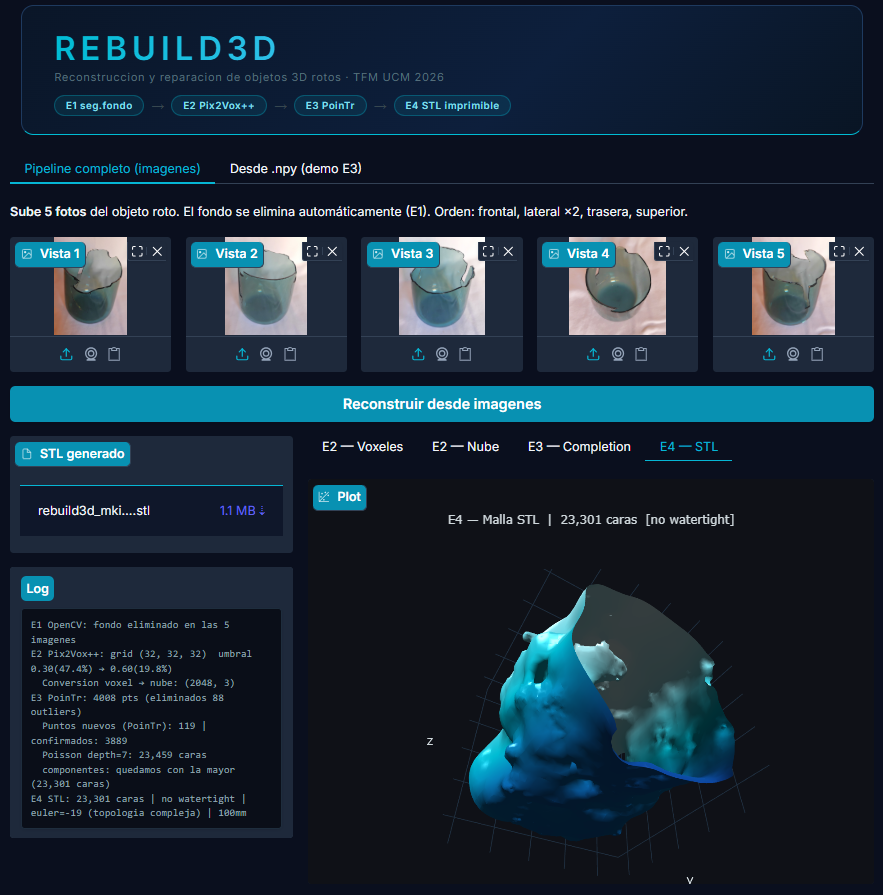
\includegraphics[width=\linewidth]{imagenes/figura_app_rebuild3d_1}
    \caption{Pipeline completo desde im\'agenes: cinco fotograf\'ias
             de una taza rota pasan por E1--E4 hasta el STL final.}
    \label{fig:app_rebuild3d_imgs}
  \end{subfigure}
  \hfill
  \begin{subfigure}[b]{0.48\linewidth}
    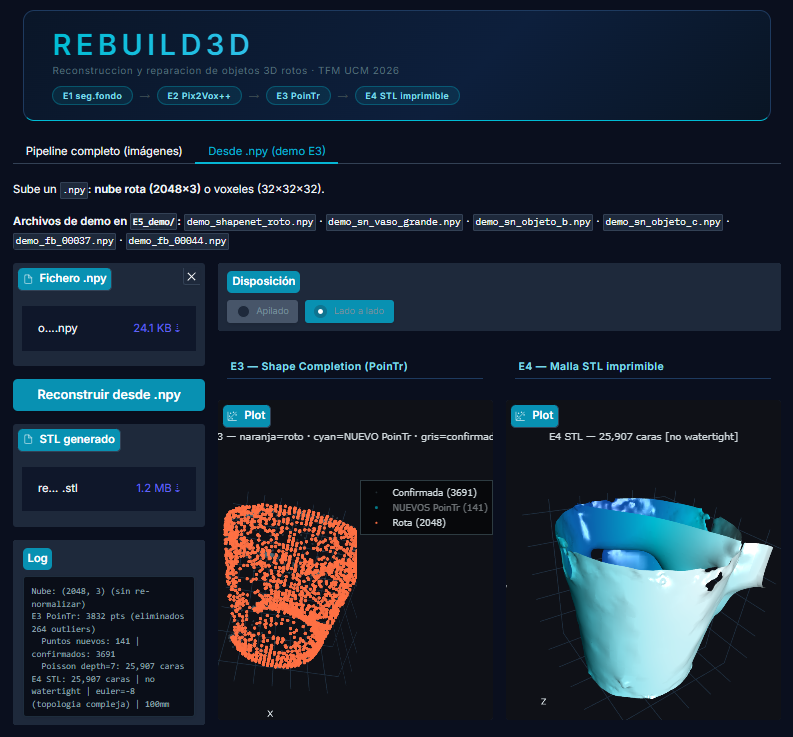
\includegraphics[width=\linewidth]{imagenes/figura_app_rebuild3d_2}
    \caption{Modo desde \texttt{.npy}: nube de puntos pre-extra\'ida
             enviada directamente a E3 (PoinTr) y E4 (STL).}
    \label{fig:app_rebuild3d_npy}
  \end{subfigure}
  \caption{Interfaz de REBUILD3D\@. Visualizaci\'on 3D interactiva por etapa
           y layout configurable (apilado o lado a lado).
           El STL es descargable directamente desde la interfaz.}
  \label{fig:app_rebuild3d}
\end{figure}

El pipeline completo (desde las cinco fotos hasta el archivo STL descargable)
se ejecuta en un único clic y tarda menos de 90 segundos en Google Colab con GPU~A100.
La aplicación se encuentra en fase beta: el rendimiento sobre fotos reales está limitado
por la brecha entre los datos sintéticos de entrenamiento y las condiciones reales de
captura, limitación descrita en detalle en la Sección~\ref{sec:limitaciones}.

% ============================================================
% ── Bibliografía ─────────────────────────────────────────────────────────────
% ============================================================
\clearpage
\bibliographystyle{apalike}
\bibliography{referencias}
\end{document}



